% PVK resources: https://polybox.ethz.ch/index.php/s/FQI5tkf1kabHnhB
% PW: SD2022
%
%
\documentclass[a4paper,10pt,landscape]{scrartcl}
\usepackage{algorithm}
\usepackage{algpseudocode}
\usepackage{multirow}
\usepackage{graphicx}
\usepackage{wrapfig}
\usepackage{tabularx}
\usepackage[table]{xcolor}
% \usepackage{svg}
% \usepackage{svg-extract}
% \svgsetup{clean=true}
\usepackage{scrlfile}
\usepackage[export]{adjustbox}
\PreventPackageFromLoading{svg}
% set margins
% \usepackage[margin=0cm]{geometry}
\usepackage{mdframed}



% for a more readable preamble
% document setup
\usepackage[margin=3mm,landscape]{geometry} % margin = .. total={280mm,190 mm} % in geometry for defined size/ratio
\usepackage{multicol,multirow}
\usepackage[utf8]{inputenc} % not strictly necessary, but sets utf8

% enable colors
\usepackage{xcolor,color} % standard colors (blue, red, etc.https://www.namsu.de/Extra/pakete/Xcolor.html )

% multicol settings
\setlength{\premulticols}{1pt}
\setlength{\postmulticols}{1pt}
\setlength{\multicolsep}{1pt}
\setlength{\columnsep}{5pt}
\setlength{\columnseprule}{1pt}
\def\columnseprulecolor{\color{black}}

% language
\usepackage[english]{babel} %choose your language

% for images
\usepackage{graphicx}
\graphicspath{ {./images/} }

% Images combined with texts
\usepackage{wrapfig}

% some AsmTeX options
\usepackage{amscd, amsmath,amssymb}

% more fine control for lists
\usepackage{enumitem}

% multiple line comments and testing text
\usepackage{verbatim} % \begin{comment} \end{comment} 
\usepackage{blindtext} % inserts lorem ipsum like text

% hyperlinks (has to be after titlesec, else we get errors
\usepackage[colorlinks=true,citecolor=blue,linkcolor=blue]{hyperref}

% svg support
\usepackage[clean]{svg}
% colors
\usepackage{color,xcolor}
\definecolor{section}{HTML}{40916c}
\definecolor{subsection}{HTML}{52b788}
\definecolor{subsubsection}{HTML}{74c69d}
\definecolor{titletext}{RGB}{0,0,0}

% colored box for section
\setkomafont{section}{\mysection}
\newcommand{\mysection}[1]{%
    \setlength{\fboxsep}{0cm}%already boxed
    \colorbox{section}{%
        \begin{minipage}{\linewidth}%
            \vspace*{2pt}%Space before
            \hspace{2pt}%left indent
            #1
            \vspace*{2pt}%Space after
        \end{minipage}%
    }}
% colored box for subsection
\setkomafont{subsection}{\mysubsection}
\newcommand{\mysubsection}[1]{%
    \setlength{\fboxsep}{0cm}%already boxed
    \colorbox{subsection}{%
        \begin{minipage}{\linewidth}%
            \vspace*{2pt}%Space before
            \hspace{2pt}%left indent
            #1
            \vspace*{2pt}%Space after
        \end{minipage}%
    }}
% colored box for subsection
\setkomafont{subsubsection}{\mysubsubsection}
\newcommand{\mysubsubsection}[1]{%
    \setlength{\fboxsep}{0cm}%already boxed
    \colorbox{subsubsection}{%
        \begin{minipage}{\linewidth}%
            \vspace*{2pt}%Space before
            \hspace{2pt}%left indent
            #1
            \vspace*{2pt}%Space after
        \end{minipage}%
    }}

% decrease wasted space in title
\RedeclareSectionCommand[
  %runin=false,
  afterindent=false,
  beforeskip=.25\baselineskip,
  afterskip=.25\baselineskip]{section}
\RedeclareSectionCommand[
  %runin=false,
  afterindent=false,
  beforeskip=.25\baselineskip,
  afterskip=.25\baselineskip]{subsection}
\RedeclareSectionCommand[
  %runin=false,
  afterindent=false,
  beforeskip=.2\baselineskip,
  afterskip=.25\baselineskip]{subsubsection}
\RedeclareSectionCommand[
  runin=true,
  %afterindent=false,
  beforeskip=.25\baselineskip,
  afterskip=1em]{paragraph}
\RedeclareSectionCommand[
  runin=true,
  %afterindent=false,
  beforeskip=.5\baselineskip,
  afterskip=1em]{subparagraph}

% set the size of a section
\usepackage{parskip}
\setlength{\parindent}{0pt}
\setlength{\parskip}{0pt plus 0.5ex}

% un-comment to hide the section numbering
%\setcounter{secnumdepth}{0} 
%-----------------------------------------------------%
% for colours
\usepackage{color}
% from code expert "ce_"
\definecolor{ce_yellow}{HTML}{228B22}
\definecolor{ce_gray}{rgb}{0.459,0.443,0.369}
\definecolor{ce_lime}{rgb}{0.459,0.816,0.180}
\definecolor{ce_pink}{rgb}{0.976,0.149,0.447}
\definecolor{ce_cyan}{rgb}{0.40,0.851,0.937}
\definecolor{ce_violet}{rgb}{0.545,0.506,1.00}
\definecolor{ce_back}{rgb}{1,1,1}
\definecolor{ce_white}{rgb}{0.15,0.15,0.12}
%----------------------------------------------------%
% as close to CodeExpert as i could get it
\usepackage{listings}

\lstdefinestyle{CodeExpert}{
    language=C++,
    basicstyle=\ttfamily\linespread{0.8}\color{ce_white},
    numbers=none,
    aboveskip=0mm,
    belowskip=0mm,
    frame = none,
    numberstyle=\tiny\color{ce_grey},
    backgroundcolor = \color{ce_back},
    keywordstyle=\color{ce_cyan},
    commentstyle=\color{ce_gray},
    stringstyle=\color{ce_yellow},
    morecomment=[n][\color{ce_pink}]{\#}{\ },
    literate=
    *{./}{{{\color{ce_pink}./}}}2
    {.^}{{{\color{ce_pink}.\^{}}}}2
    {=}{{{\color{ce_pink}=}}}1
    {+}{{{\color{ce_pink}+}}}1
    {*}{{{\color{ce_pink}*}}}1
    {-}{{{\color{ce_pink}-}}}1
    {&}{{{\color{ce_pink}&}}}1
    {<<}{{{\color{ce_pink}<<}}}2
    {>>}{{{\color{ce_pink}>>}}}2
    {<}{{{\color{ce_pink}<}}}1
    {>}{{{\color{ce_pink}>}}}1
    {->}{{{\color{ce_pink}->}}}2
    {1}{{{\color{ce_violet}1}}}1
    {2}{{{\color{ce_violet}2}}}1
    {3}{{{\color{ce_violet}3}}}1
    {4}{{{\color{ce_violet}4}}}1
    {5}{{{\color{ce_violet}5}}}1
    {6}{{{\color{ce_violet}6}}}1
    {7}{{{\color{ce_violet}7}}}1
    {8}{{{\color{ce_violet}8}}}1
    {9}{{{\color{ce_violet}9}}}1
    {0}{{{\color{ce_violet}0}}}1
    {this}{{{\color{ce_lime}this}}}1
    {if}{{{\color{ce_pink}if}}}1
    {do}{{{\color{ce_pink}do}}}1
    {for}{{{\color{ce_pink}for}}}1
    {else}{{{\color{ce_pink}else}}}1
    {then}{{{\color{ce_pink}then}}}1
    {break}{{{\color{ce_pink}break}}}1
    {continue}{{{\color{ce_pink}continue}}}1
    {public}{{{\color{ce_pink}public}}}1
    {private}{{{\color{ce_pink}private}}}1
    {while}{{{\color{ce_pink}while}}}1
    {continue}{{{\color{ce_pink}continue}}}1
    {nullptr}{{{\color{ce_violet}nullptr}}}1
    {NULL}{{{\color{ce_violet}NULL}}}1,
}

\lstset%
    {
    basicstyle=\ttfamily,
    frame=tb,
    aboveskip=1mm,
    belowskip=1mm,
    showstringspaces=true,
    columns=flexible,
    breaklines=true,
    breakatwhitespace=true,
    tabsize=2,
}
%Mathematik-Pakete
\usepackage{amsmath, amstext, amssymb, mathtools, esint, polynom}
\usepackage{bm}
\allowdisplaybreaks %Seitenumbruch in align-Umgebung erlauben
%

%Definition der Umgebung "example"
\newenvironment {example}
				{\begin{itshape} \begin{small}}
				{\end{small} \end{itshape}}
%				
%Definition der Umgebung "annotation"		
\newenvironment {annotation}[1]
				{\begin{itshape} \begin{small} \textbf{#1} \begin{itemize}}
				{\end{itemize} \end{small} \end{itshape}}
%				
%Definition der Umgebung "eq"
\newenvironment {eq}
				{\begin{equation*}}
				{\end{equation*}}
%
% Don't know what this does
\providecommand{\diff}{\mathop{} \! \mathrm{d}}
\DeclareMathOperator{\rot}{rot}
\DeclareMathOperator{\divg}{div}
% -------------------------------------------
\title{PSA Summary}
\subtitle{HS24 ETH Zurich}
\author{Carl von Holly-P.}
% \date{\today}
%
\begin{document}
\begin{multicols*}{3}
%
\maketitle
\vspace{-1.2cm}
\section{Basics}
resistance and reactance:
$z=r+jx=\frac{1}{y} = \frac{1}{g + jb}$ \\
conductance and susceptance: $g=\frac{r}{r^2 + x^2}$, $b=\frac{x}{r^2 + x^2}$ \\
per unit: $r=r^{pu}\cdot r_{B}\quad\left[\mathrm{p.u.}\right]\cdot\left[\mathrm{\frac{\Omega}{p.u.}}\right]$, $I_B=\frac{S_B}{\sqrt{3}\cdot U_B}$
\section{Components}
\subsection{Transmission line}
$\underline{I}_{k m}=\left(a_{k m}^2 \underline{E}_k-t_{k m}^* t_{m k} \underline{E}_m\right) y_{k m}+y_{k m}^{S h} a_{k m}^2 \underline{E}_k$

\subsection{Phase shifting transformers}
\begin{figure}[H]
    \centering
    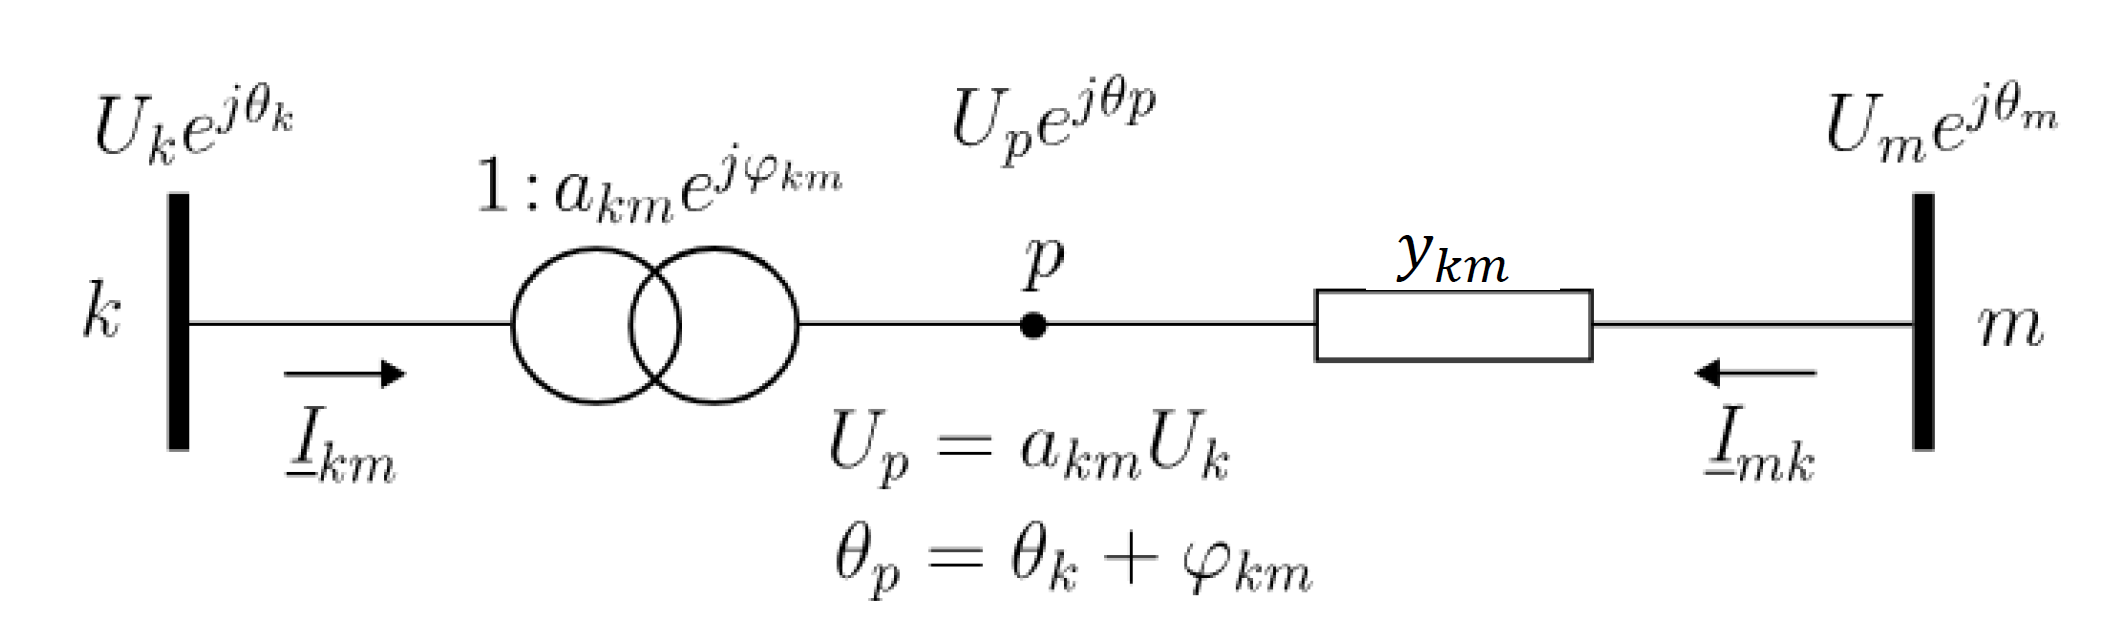
\includegraphics[width=\linewidth]{src/image.png}
\end{figure}
$\binom{\underline{I}_{k m}}{\underline{I}_{m k}}=\left(\begin{array}{cc}a_{k m}^2 y_{k m} & -t_{k m}^* y_{k m} \\ -t_{k m} y_{k m} & y_{k m}\end{array}\right)\binom{\underline{E}_k}{\underline{E}_m}$ \\
$\begin{aligned} P_{k m} & =a_{k m}^2 U_k^2 g_{k m}-a_{k m} U_k U_m g_{k m} \cos \left(\theta_{k m}+\varphi_{k m}\right) \\ & -a_{k m} U_k U_m b_{k m} \sin \left(\theta_{k m}+\varphi_{k m}\right)\end{aligned}$
$\begin{aligned} Q_{k m} & =-a_{k m}^2 U_k^2 b_{k m}+a_{k m} U_k U_m b_{k m} \cos \left(\theta_{k m}+\varphi_{k m}\right) \\ & -a_{k m} U_k U_m g_{k m} \sin \left(\theta_{k m}+\varphi_{k m}\right)\end{aligned}$ \\
where $\theta_{km}=\theta_k-\theta_m$ the voltage angle difference, $t_{km}=a_{km}e^{j\varphi_{km}}$ the transformer model, $\varphi_{km}$ the phase shift.

\subsection{power losses in line}
$P_{loss}=P_{mk}+P_{km}=g_{km}|E_k-E_m|^2$ \\
$Q_{loss}=Q_{mk}+Q_{km}=-b_{km}^{sh}(U_k^2+U_m^2)-b_{km}|E_k-E_m|^2$

\subsection{Unified Branch Model}
idea: combine all devices in one model. \\
Transmission line: $a_{km}=a_{mk}=1$, $\varphi_{km}=\varphi_{mk}=0$. \\
Transformers: $y^{sh}_{km}=y^{sh}_{mk}=0$, $a_{mk}=1$, $\varphi_{mk}=0$.
\begin{figure}[H]
    \centering
    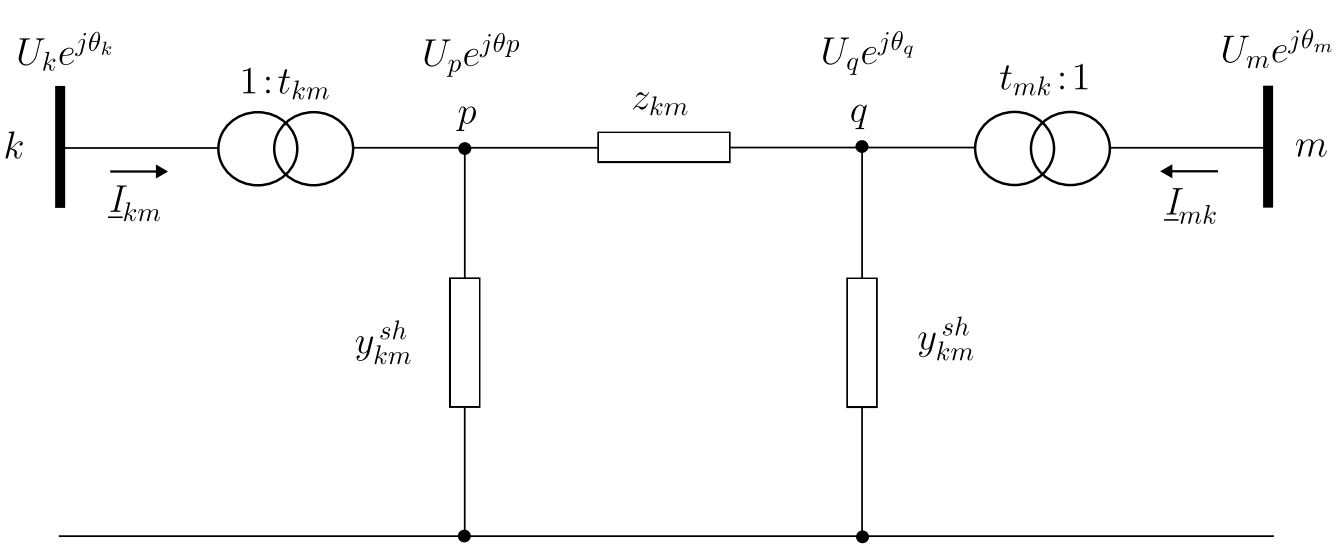
\includegraphics[width=1\linewidth]{src/ubm.png}
\end{figure}
$\binom{\underline{I}_{k m}}{\underline{I}_{m k}}=\left(\begin{array}{cc}a_{k m}^2\left(y_{k m}+y_{k m}^{s h}\right) & -t_{k m}^* t_{m k} y_{k m} \\ -t_{m k}^* t_{k m} y_{k m} & a_{m k}^2\left(y_{k m}+y_{k m}^{s h}\right)\end{array}\right)\binom{\underline{E}_k}{\underline{E}_m}$ \\
$\begin{aligned} P_{k m} & =\left(a_{k m} U_k\right)^2 g_{k m} \\ & -\left(a_{k m} U_k\right)\left(a_{m k} U_m\right) g_{k m} \cos \left(\theta_{k m}+\varphi_{k m}-\varphi_{m k}\right) \\ & -\left(a_{k m} U_k\right)\left(a_{m k} U_m\right) b_{k m} \sin \left(\theta_{k m}+\varphi_{k m}-\varphi_{m k}\right)\end{aligned}$ \\
$\begin{aligned} Q_{k m} & =-\left(a_{k m} U_k\right)^2\left(b_{k m}+b_{k m}^{s h}\right) \\ & +\left(a_{k m} U_k\right)\left(a_{m k} U_m\right) b_{k m} \cos \left(\theta_{k m}+\varphi_{k m}-\varphi_{m k}\right) \\ & -\left(a_{k m} U_k\right)\left(a_{m k} U_m\right) g_{k m} \sin \left(\theta_{k m}+\varphi_{k m}-\varphi_{m k}\right)\end{aligned}$


\subsection{shunt elements}
$I_k^{sh}=-y_k^{sh}E_k$ (meaning pos. current for current \textit{into} bus $k$)

\subsection{loads}
Assume load active \& reactive power is constant.
\subsection{generators}
\subsubsection{capability curve}
$S_g=P_g + jQ_g$ is limited
\begin{itemize}
    \item in $P_{g,max}$ by stator current heating limit (max. losses in armature $R_t|I_t|^2$
    \item in $Q_{g,max}$ by field current heating limit
    \item in $Q_{g,min}$ by stator end region heating limit (eddy currents leading to heat)
\end{itemize}

\subsection{admittance matrix}
nodal admittance matrix: $\mathbf{Y=G+jB}\Rightarrow\mathbf{I=YE}$ \\
with elements
$Y_{km} = -t_{km}^*t_{mk}y_{km}:=G_{km} + jB_{km}$ \\
$Y_{kk} = y_k^{sh}+\underset{m\in\Omega_k}{\sum}a_{km}^2(y_{km}^{sh} + y_{km}):=G_{kk} + jB_{kk}$ \\
characteristics: \textit{sparse} and generally \textit{symmetric} (not in case of phase-shifting-trafo)

\section{Power Flow Computation}
variables: $P_k,Q_k,U_k,\theta_k$ (redundancy: 2 variables) \\
$P_k,Q_k$ are the active and reactive power injections at bus $k$: 
$P_k=P_{G_{k}} - P_{L_{k}}$ \\
$=U_k^2G_{kk}+U_k \sum_{m \in K} U_m\left(G_{k m} \cos \theta_{k m}+B_{k m} \sin \theta_{k m}\right)$ and \\
$Q_k =  -U_k^2B_{kk} + U_k \sum_{m \in K} U_m\left(G_{k m} \sin \theta_{k m}-B_{k m} \cos \theta_{k m}\right)$.

\subsection{Bus Types}
\vspace{-.5cm}
\begin{table}[H]
    \centering
    \begin{tabular}{c|c|c|c|c}
         Bus type&  a.k.a.& known's & equal. constr. & \\ \hline
         slack&  & $U_k,\theta_k=0$ & $U=$ const., $\theta_k=0$ & \\
         PQ&  load& $P_k,Q_k$ & $P,Q$ balance & \\
         PU&  gen.& $P_k,Q_k$ & $P$ balance, $U=$ const. &
    \end{tabular}
\end{table}
\vspace{-.5cm}

\subsection{DC Power Flow}
assumptions:
\begin{itemize}
    \item $|U_{bus}|=1$ at all buses, neglect shunt elements
    \item small $\theta_{km}\Rightarrow \cos(\theta_{km})\approx1, \sin(\theta_{km})\approx \theta$
    \item lossless transmission lines \& power transformers
\end{itemize}
equations for tr.-line, in-phase-trafo, phase shifter:
$$P_{km}=\frac{\theta_{km}}{x_{km}} \quad P_{km}=\frac{\theta_{km}}{x_{km}/a_{km}} \quad P_{km}=\frac{\theta_{km}+\varphi_{km}}{x_{km}}$$
\subsubsection{DC Load Flow}
$$P_k=P_{G_{k}}-P_{L_{k}} = \underset{m\in\Omega_k}{\sum}\frac{\theta_k-\theta_m}{x_{km}}=B_{kk}'\theta_k + \underset{m\in\Omega_k}{\sum}B_{km}'\theta_m$$
$$\Rightarrow \mathbf{P=B'\theta}, \quad \mathbf{B'_{kj}}=\sum_{m\in\Omega_k}x_{km}^{-1} \text{ if } k=j, \text{else } -x_{km}^{-1}$$
Row $i$ may have to be deleted as $\theta_i=0$ is slack/reference bus. \\
With $\mathbf{P}$ vector of net injections, $\mathbf{B'}$ nodal admittance matrix. If there are phase shifting transformers: $\mathbf{P=B'\theta-P_{pst}}$

\subsection{Gauss(-Seidel) approach}
starting from $S_k=\underline{E}_k \sum_{m \in K} Y_{k m}^* \underline{E}_m^*, \quad k=1,2, \ldots, N$ \\
$E_k=U_k e^{j\theta_k}$ can be rewritten as
$$\underline{E}_k=\frac{1}{Y_{k k}}\left[\frac{S_k^*}{\underline{E}_k^*}-\sum_{m \in \Omega_k} Y_{k m} \underline{E}_m\right]=h_k(E_1,\dots,E_N)$$
then we can combine $\mathbf{x=h(x)}$ and iteratively solve $\mathbf{x^{(\nu+1)}=h(x^{(\nu)})}$
starting from $\mathbf{x^{(0)}}=[E_1^{(0)} \dots E_N^{(0)}]^T$. \\
flat start: $E_i^{(0)}=1\quad\forall i$.\\
In Gauss-Seidel (vs Gauss): use most recent values, e.g. $E_k^{(\nu+1)}=h_k(E_1^{(\nu+1)} \dots E_{k-1}^{(\nu+1)} E_k^{(\nu)} \dots E_N^{(\nu)})$
characteristics :
\begin{itemize} 
    \item convergence Gauss-Seidel faster then Gauss
    \item but Gauss-Seidel cannot be parallelize
\end{itemize}

\subsection{Newton-Raphson}
has quadratic convergence near $x^*$. algorithm:
\begin{enumerate}
    \item set $\nu=0,\mathbf{x^{(0)}}$
    \item compute $\mathbf{f(x^{(\nu)})}$
    \item test convergence: if $|f_i(|\mathbf{x^{(\nu)}}|)\leq \epsilon\quad\forall i$: stop
    \item solve $\mathbf{f(x^{(\nu)}) + J(x^{(\nu)})\Delta x^{(\nu)}=0}$ for $\mathbf{\Delta x^{(\nu)}}$
    \item $\mathbf{x^{(\nu+1)} = x^{(\nu)} + \Delta x^{(\nu)}}$
    \item $\nu\leftarrow \nu+1$ and go to 2.
\end{enumerate}
with $\mathrm{x}=\binom{\boldsymbol{\theta}}{\mathbf{U}}$, where $\mathbf{U}$ are the magnitudes of the PQ buses. 
$\mathbf{f}(\mathbf{x})=\binom{\Delta \mathbf{P}(\mathrm{x})}{\Delta \mathbf{Q}(\mathrm{x})}=\binom{\mathbf{P}(\mathrm{x})-\mathbf{P}^{(\mathrm{s})}}{\mathbf{Q}(\mathrm{x})-\mathbf{Q}^{(\mathrm{s})}}$
where $\mathbf{P}^{(\mathrm{s})}$ are the known power injections into bus $k$ from generators and loads.

\subsection{$P\theta-QU$ Decoupling}
simplifying to $\theta_{km}=0$ ($J$ becomes diagonal, easier to compute, more inaccurate.)

\subsection{structure and levels}
from level 1 (high V transmission, 220-380 kV) to 7 (local distribution grid).
\subsubsection{level 5: regional distribution grid}
mid voltages 6kV - 30kV. suplly small towns, industrial enterprises, ... Weakly meshed grid topology. Small power plants. Has transformers to lower levels.
\subsubsection{level 7: local distribution grid}
Europe: phase voltage of 230V (P-P=400V). Supply all customers. Radial or weakly meshed structure. Infeed types: PV, transformers.
\subsection{properties of distribution networks}
these properties can lead to ill-conditioned system
\begin{itemize}
    \item radial/weakly meshed networks
    \item high $R/X$ ratios
    \item multiphase, unbalanced operation
    \item unbalanced distributed load
    \item distributed generation
\end{itemize}
\subsection{Power Flow Methods for Radial Grids}
advant.: faster, robuster, exploit properties above. types:
\begin{itemize}
    \item Network Reduction Methods \ref{Network Reduction Method}
    \item Backward/Forward Sweep Methods
    \item Fast decoupled Methods
\end{itemize}

\subsection{Network Reduction Method}\label{Network Reduction Method}
replacing non-linear element with linear counterpart. procedure, repeat. 2.-4. til convergence:
\begin{enumerate}
    \item initialize bus voltages $\mathbf{E}$
    \item linearize system based on $\mathbf{E}$
    \item build driving point equivalent circuit at each bus
    \item compute all voltages and currents
\end{enumerate}
\subsubsection{linearization} 
generators and PQ loads. Thus: \\ 
$\underline{I}_k(\underline{E}_k) = \hat{\underline{I}}_k+\hat{Y}\underline{E}_k\approx \hat{\underline{I}}_k=\left(\frac{P_k+jQ_k}{\underline{E}_k}\right)^2$ \\
\subsubsection{build driving point equivalent circuit at each bus}
Norton equivalent at bus $k$: aggregate admittances and current sources into the form (left): $\underline{I}_k = \underline{I}_{EQk} - Y_{EQk}'\underline{E}_k$.
Now combine Norton equivalent's with the incoming branch (right): \\
\begin{figure}[H]
    \centering
    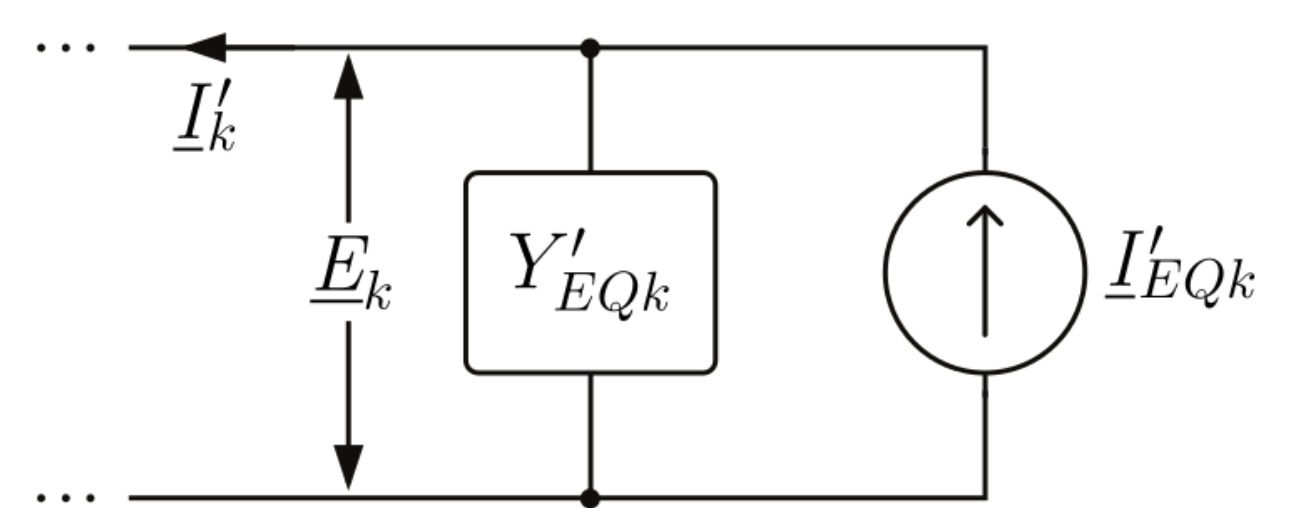
\includegraphics[width=.49\linewidth]{src/norton.png}
    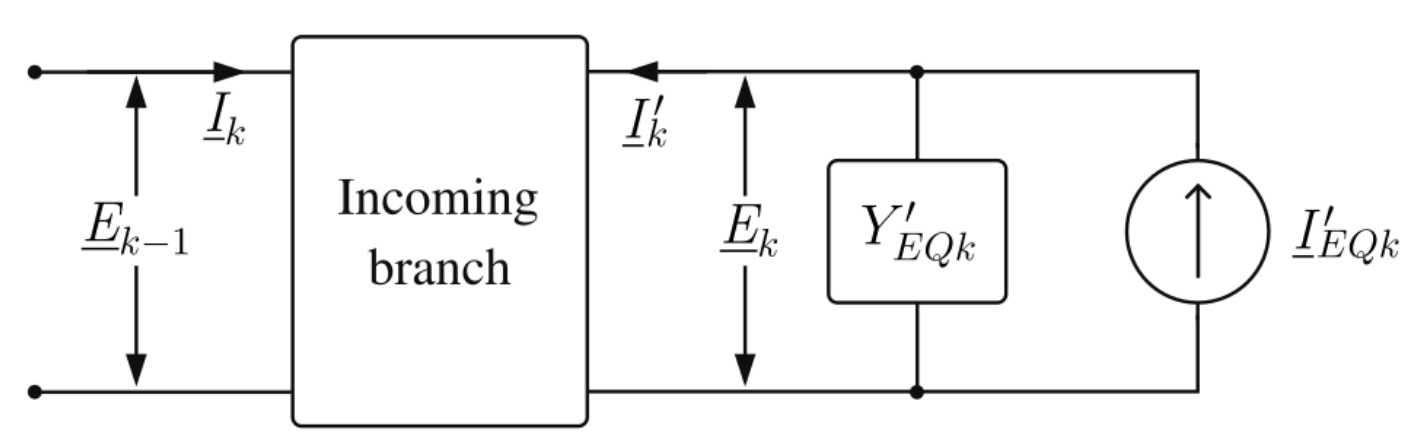
\includegraphics[width=.49\linewidth]{src/incoming_branch.png}
\end{figure}
% \begin{figure}[H]
%     \centering
    
% \end{figure}
is transformed into its driving point equivalent
% \begin{wrapfigure}{l}{0.5\linewidth}
%     \centering
%     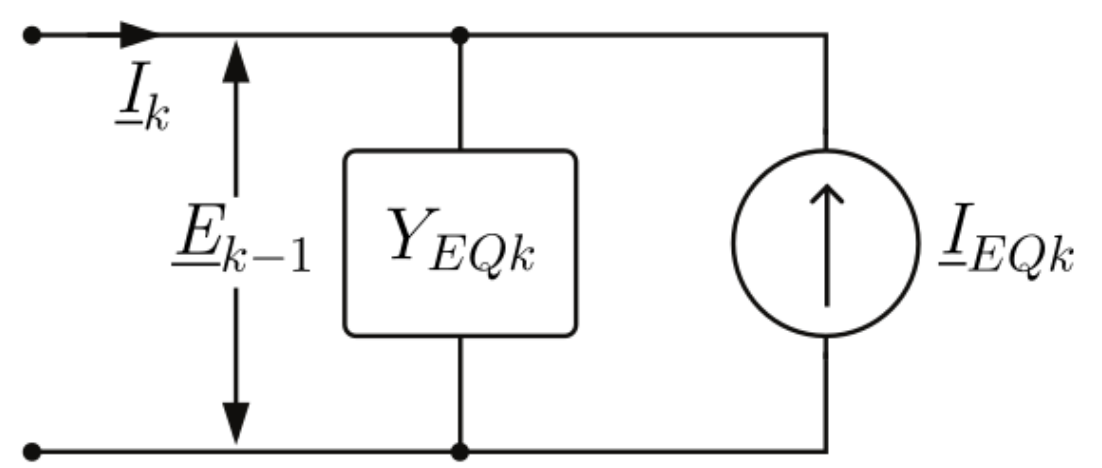
\includegraphics[width=\linewidth]{src/norton_combine.png}
% \end{wrapfigure}
% $\underline{I}_{EQk} = Y_{EQk}\underline{E}_{k-1} - \underline{I}_k$ \\
% $Y_{E Q k}=Z_k^{-1}+\frac{1}{2} Y_k-Z_k^{-1}\left(Z_k^{-1}+\frac{1}{2} Y_k+Y_{E Q k}^{\prime}\right)^{-1} Z_k^{-1}$ \\
% $\underline{I}_{E Q k}=Z_k^{-1}\left(Z_k^{-1}+\frac{1}{2} Y_k+Y_{E Q k}^{\prime}\right)^{-1} \underline{I}_{E Q k}^{\prime}$
\begin{figure}[H]
    \centering
    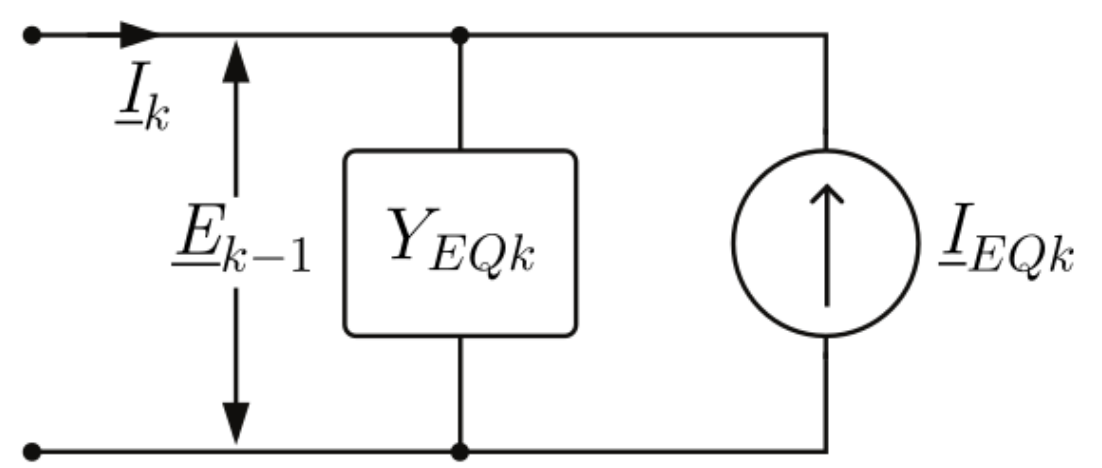
\includegraphics[width=.6\linewidth]{src/norton_combine.png}
\end{figure}
via \\
$$\begin{gathered}
\underline{I}_{EQk} = Y_{EQk}\underline{E}_{k-1} - \underline{I}_k \\
Y_{E Q k}=Z_k^{-1}+\frac{1}{2} Y_k-Z_k^{-1}\left(Z_k^{-1}+\frac{1}{2} Y_k+Y_{E Q k}^{\prime}\right)^{-1} Z_k^{-1} \\ 
\underline{I}_{E Q k}=Z_k^{-1}\left(Z_k^{-1}+\frac{1}{2} Y_k+Y_{E Q k}^{\prime}\right)^{-1} \underline{I}_{E Q k}^{\prime}\end{gathered}$$

\subsubsection{Computing Voltages and Currents}
start at first branch and iterate:
\begin{figure}[H]
    \centering
    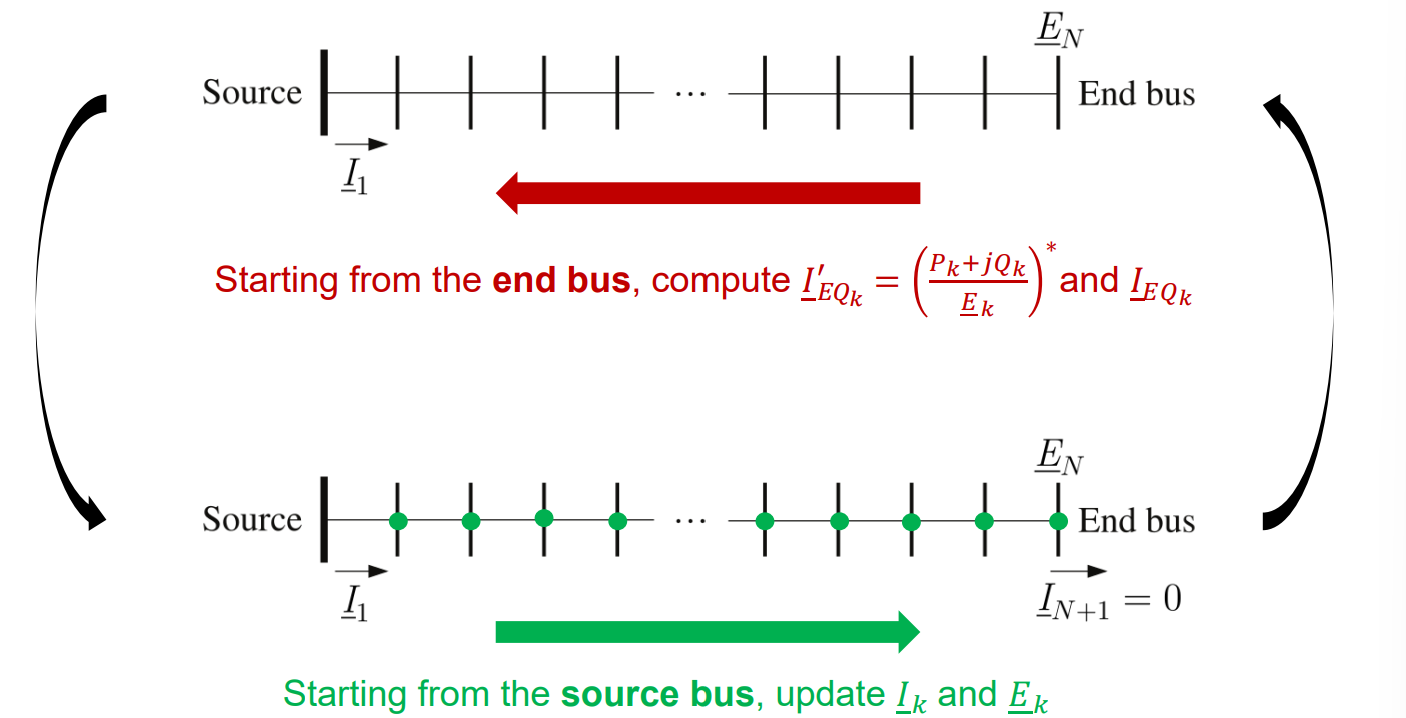
\includegraphics[width=1\linewidth]{src/network_reduction_method.png}
\end{figure}
via (starting from source bus, often $\underline{E}_1=1\angle 0, E_2=\dots$)
$$
\underline{E}_k = \underline{E}_{k-1} - Z_k \left(\underline{I}_k - \frac{Y_k}{2}\underline{E}_{k-1}\right)
$$

\subsection{Backward/Forward Sweep Methods}
based on: there is a unique path from all buses to source \\
high-level algorithm:
\begin{enumerate}
    \item initialize bus voltages $\mathbf{E}$
    \item \textbf{Backward sweep: sum $I$ with updated voltages}
    \item \textbf{Forward sweep: calculate voltage drops}
    \item repeat 2. + 3. until convergence
\end{enumerate}
Given the bus-injection to branch-current (\textbf{BIBC}) and Branch-current to bus-voltage (\textbf{BCBV}) matrices, neglecting shunt elements of lines the detailed alogithm is as follows: \\
Input: $\mathrm{BIBC}, \mathrm{BCBV}, \underline{E}_1, P_{\mathrm{inj}, k}, Q_{\mathrm{inj}, k}$ \\
Output: $\underline{I}_{\mathrm{br}, i}^{(\nu)}, \underline{E}_k^{(\nu+1)}$ for all $k \in \mathcal{N}$ and $i \in \mathcal{T}$ \\
1: initialize: $\nu=1, \underline{E}_k^{(\nu)}=1 \angle 0^{\circ}$ \\
2: while $\max \left\{\left|\underline{E}_k^{(\nu)}\right|-\left|\underline{E}_k^{(\nu-1)}\right|\right\} \geq \bar{\eta}$ do \\
3: $\quad$Backward sweep: $\underline{I}_{\mathrm{inj}, k}^{(\nu)}=\left(\frac{\left(P_{\mathrm{inj}, k}+j Q_{\mathrm{inj}, k}\right)^*}{\underline{E}_k^{(\nu) *}}\right)$ \\
4: $\quad \mathbf{I}_{\mathrm{br}}^{(\nu)}=\mathbf{BIBC} \cdot \mathbf{I}_{\mathrm{inj}}^{(\nu)}$ \\
5: $\quad$Forward sweep: $\Delta \mathbf{E}^{(\nu+1)}=\mathbf{B C B V} \cdot \mathbf{I}_{\mathrm{b r}}^{(\nu)}$ \\
6: $\quad \mathbf{E}^{(\nu+1)}=\mathbf{E}_{\text {slack }}+\Delta \mathbf{E}^{(\nu+1)}$ \\
7: $\quad \nu=\nu+1$ \\
9: return $\underline{I}_{\mathrm{br}, k}^{(\nu)}, \underline{E}_k^{(\nu+1)}$ for all $k \in \mathcal{N}$ and $i \in \mathcal{T}$ \\

\subsubsection{weakly meshed structure}
For a weakly meshed structure, the \textbf{BIBC} and \textbf{BCBV} matrices have to be adjusted, see example below:
\begin{figure}[H]
    \centering
    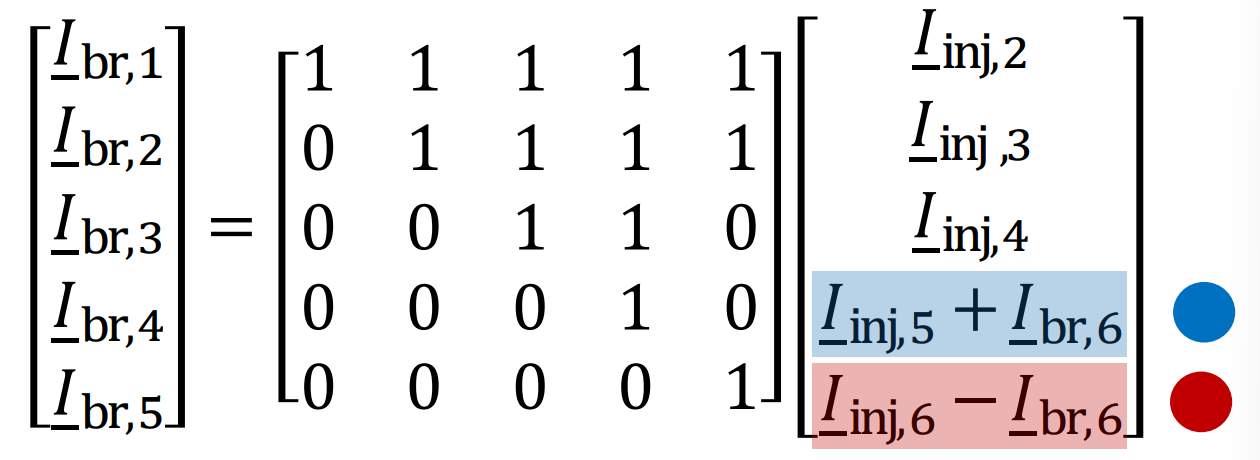
\includegraphics[width=.49\linewidth]{src/BIBC_01.png}
    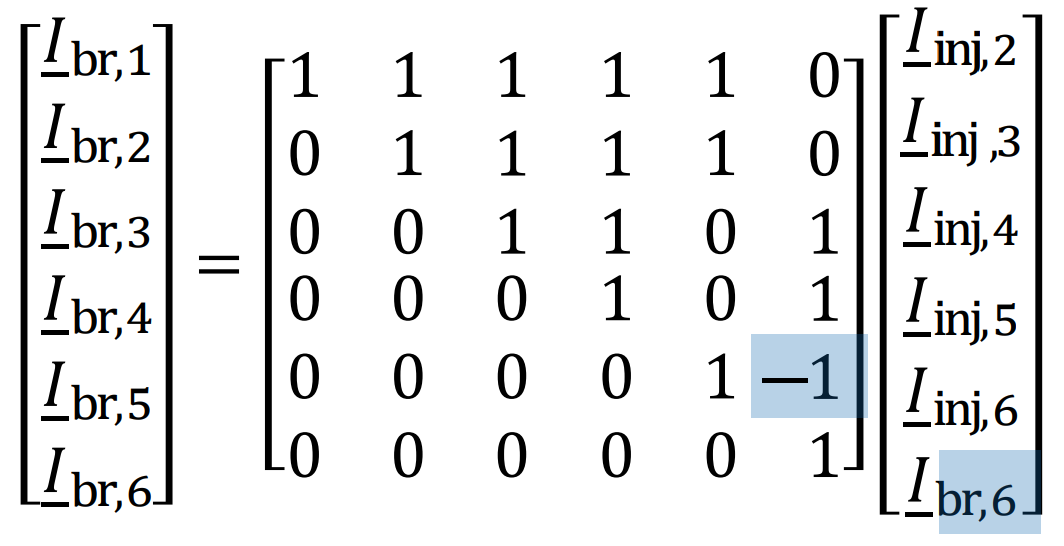
\includegraphics[width=0.49\linewidth]{src/BIBC_02.png}
\end{figure}
\begin{figure}[H]
    \centering
    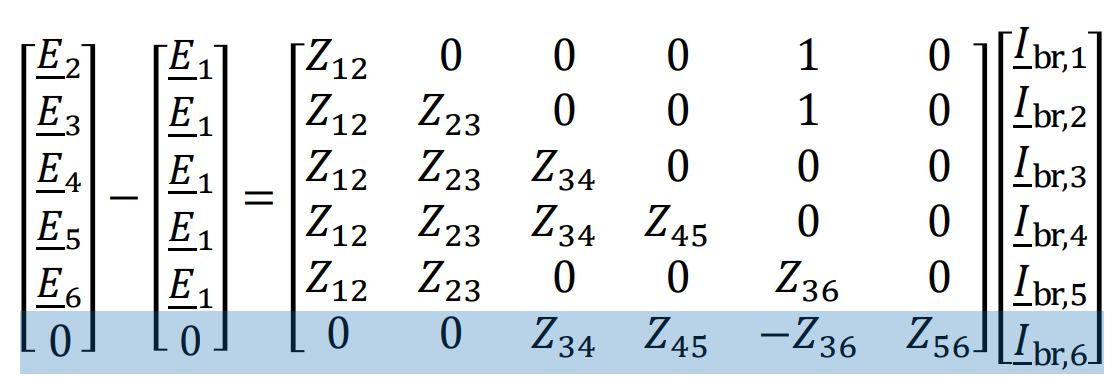
\includegraphics[width=1\linewidth]{src/BCBV.png}
\end{figure}

\begin{figure}[H]
    \centering
    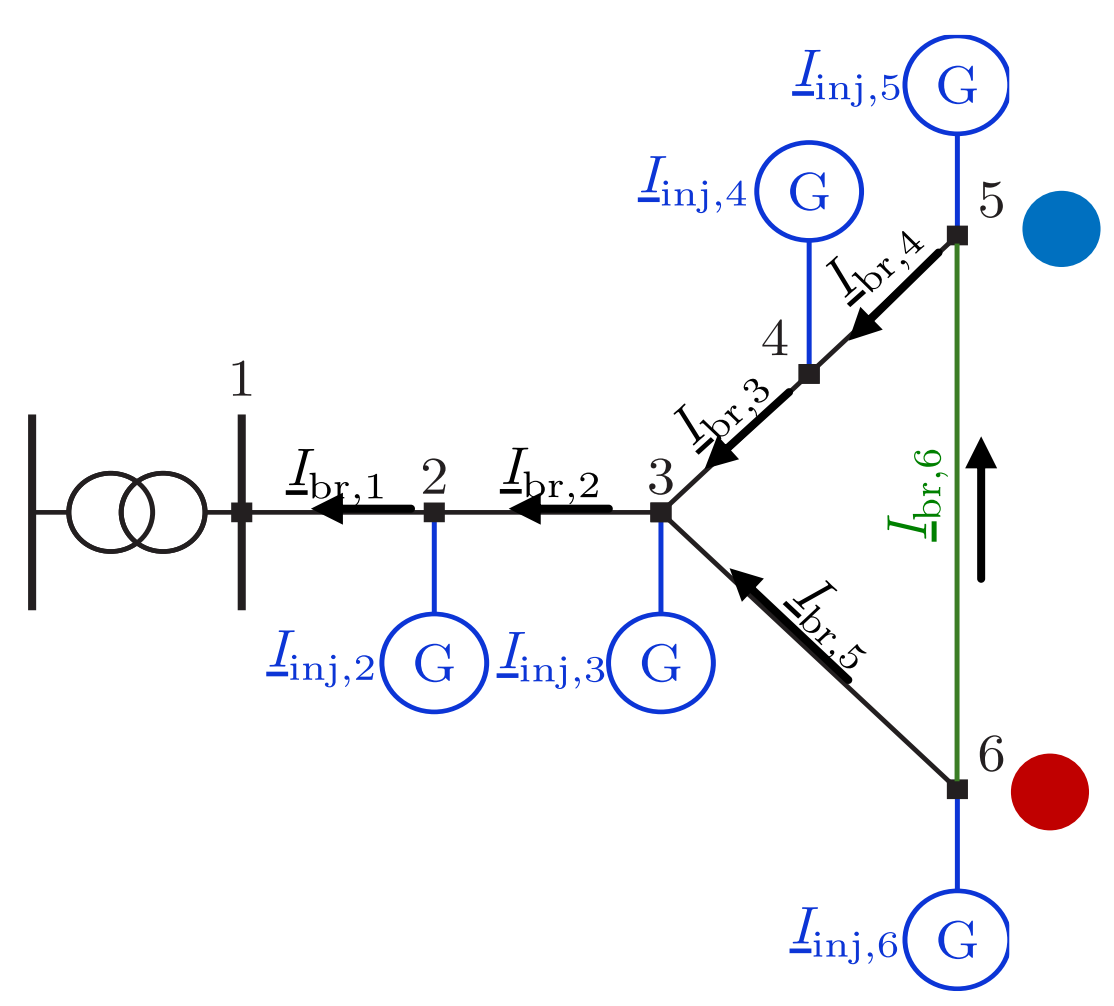
\includegraphics[width=.7\linewidth]{src/weakly_meshed.png}
\end{figure}
\vspace{-1cm}


resulting in the following equation:
\begin{equation*}
\resizebox{.9\hsize}{!}{
\left[\begin{array}{c}
\Delta \mathbf{E} \\
0
\end{array}\right]=\left[\mathbf{B C B V}_{\mathbf{m}}\right]\left[\mathbf{B I B C}_{\mathbf{m}}\right]\left[\begin{array}{c}
\mathbf{I}_{\mathbf{i n j}} \\
\underline{\mathbf{I}}_{\mathrm{br}, \mathrm{new}}
\end{array}\right]=\left[\begin{array}{cc}
\mathbf{A} & \mathbf{M}^{\mathrm{T}} \\
\mathbf{M} & \mathbf{N}
\end{array}\right]\left[\begin{array}{c}
\mathbf{I}_{\mathbf{i n j}} \\
\underline{I}_{\mathrm{brr}, \mathrm{new}}
\end{array}\right]
}
\end{equation*}
% $$\left[\begin{array}{c}
% \Delta \mathbf{E} \\
% 0
% \end{array}\right]=\left[\mathbf{B C B V}_{\mathbf{m}}\right]\left[\mathbf{B I B C}_{\mathbf{m}}\right]\left[\begin{array}{c}
% \mathbf{I}_{\mathbf{i n j}} \\
% \underline{\mathbf{I}}_{\mathrm{br}, \mathrm{new}}
% \end{array}\right]=\left[\begin{array}{cc}
% \mathbf{A} & \mathbf{M}^{\mathrm{T}} \\
% \mathbf{M} & \mathbf{N}
% \end{array}\right]\left[\begin{array}{c}
% \mathbf{I}_{\mathbf{i n j}} \\
% \underline{I}_{\mathrm{brr}, \mathrm{new}}
% \end{array}\right]$$
then using Kron reduction
$$[\Delta \mathbf{E} ]=[\mathbf{A-M^TN^{-1}M}][\mathbf{I_{inj}}]$$

\subsubsection{Full Model of BFS Power Flow}
shunts are not neglected, computation more complicated.  \\
define $g_k(\underline{\omega}_k): (\underline{E}_k, 0) \rightarrow (\underline{E}_{k-1}, \underline{I}_k)$ as follows:\\
\begin{mdframed}
\textbf{1. comp. $\underline{\tilde{I}}_{Gk}, \underline{\tilde{I}}_{Ck}, \underline{\tilde{I}}_{Lk}$ from $\underline{E}_{k}$}
\begin{figure}[H]
    \centering
    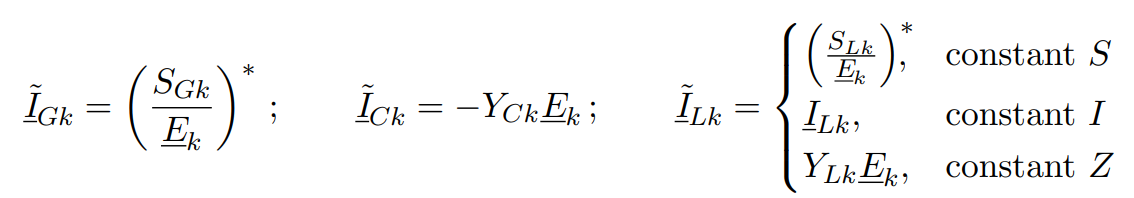
\includegraphics[width=1\linewidth]{src/full_NRM_1.png}
\end{figure}
\textbf{2. comp. $I_k'$ via KCL at bus $k$: \\ $\quad I_k'=\underline{\tilde{I}}_{Gk}+\underline{\tilde{I}}_{Ck}-\underline{\tilde{I}}_{Lk}-\underline{I}_{k+1}-\sum_{j\in A_k}\underline{I}_j$} \\
\textbf{3. comp. $\underline{\tilde{E}}_{k}$ from}
$\quad \underline{\tilde{E}}_{k-1}=\underline{E}_k+Z_k\left(\frac{1}{2} Y_k \underline{E}_k-\underline{I}_k^{\prime}\right), $ \\
$\tilde{I}_k=\frac{1}{2} Y_k\left(\underline{E}_k+\underline{\tilde{E}}_{k-1}\right)-\underline{I}_k^{\prime}$ \\
\end{mdframed}
then iteratively apply to compute:
$$\underline{\omega}_0=\left[\begin{array}{c}
\underline{E}_0 \\
\underline{I}_1
\end{array}\right]=g_1\left(\underline{\omega}_1\right)=g_1 \circ \ldots \circ g_{N-1} \circ g_N\left(\left[\begin{array}{c}
\underline{E}_N \\
\mathbf{0}
\end{array}\right]\right)$$
very similar, the forward sweep (see detail appendix \ref{full_NRM_f}) will compute :
$$\underline{\omega}_N=\left[\begin{array}{c}
\underline{U}_N \\
\underline{I}_{N+1}
\end{array}\right]=f_N\left(\underline{\omega}_{N-1}\right)=f_N \circ \ldots \circ f_2 \circ f_1\left(\left[\begin{array}{c}
\underline{E}_0^* \\
\underline{I}_1
\end{array}\right]\right)$$
% \begin{enumerate}
%     \item comp. $\underline{\tilde{E}}_{k}$ from
% \end{enumerate}

% new column
\vfill\null
\columnbreak


\section{Synchronous Machine}
\begin{wrapfigure}{l}{0.75\linewidth}
    \centering
    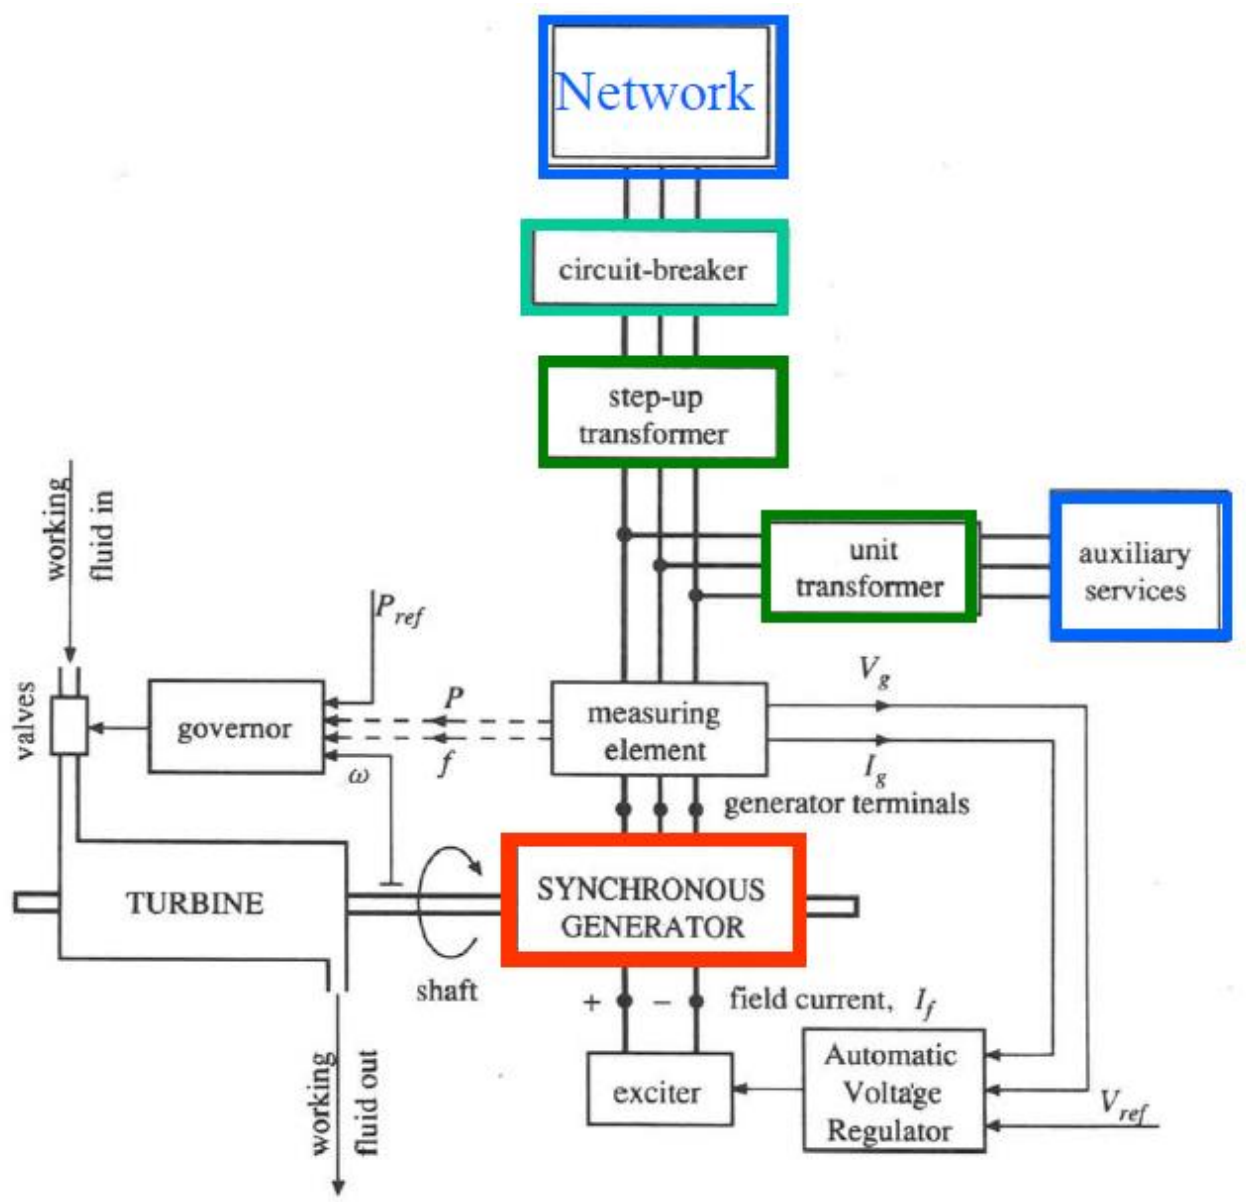
\includegraphics[width=\linewidth]{src/sync_machine_in_network.png}
\end{wrapfigure}
\textit{stator}: 3 identical phase windings \\
\textit{rotor}: rotates at $\omega_r=N=\frac{2\cdot 60}{p}f$ where $p$ \#poles, $f$ grid freq. has 1 field winding: DC $i_f$

% \subsection{types}
\textbf{round-rotor (rr)}:
$p=\{2,4\}\rightarrow$ high speed. steam and gas turbines. up to 1.8GVA. horizontal op. 

\textbf{salient pole (sp)}:
$p>4\rightarrow$ lower speed. hydro turbines. up to 800 MVA. vertical operation. 

\subsection{principle of operation}
\begin{itemize}
    \item $I_F$ excites rotor winding $\rightarrow$ rotating magnetic field $B_r$
    \item flux $\Phi_{B_{r}}$ induces $\mathrm{emf}$ in stator $\rightarrow$ $V$ in phases $\rightarrow$ AC current $i_a,i_b,i_c$ $\rightarrow$ rotating field thus magnetic torque $T_e$
    \item $T_e$ opposes mech. torque $T_m$ of turbine: $T_m=T_e$
\end{itemize}

\subsection{inductance's}
self-inductances stator: $L_s=L_{aa}=L_{bb}=L_{cc}$. mutual: $L_{ab}=L_{bc}=L_{ca}=-M_S$. Self-inductance rotor: $L_{FF}$. mutual inductances rotor/stator $L_{xf}=M_f\cos(\theta_d-\gamma_x)$ where $\gamma_x=\{0,120^\circ,240^\circ\}$ for $x=\{a,b,c\}$

\subsection{phase equations}
for phase $x$, $u_x=-R i_x - (L_s+M_S)\frac{di_x}{dt}+e_x'$ where $e_{x'}=\omega M_fI_f\sin(\omega t+\theta_{d0}-\rho_x)=\sqrt{2}|E_i|\cos (\omega t+\theta)$ is the \textit{internal voltage source}. $i_x$ lags $\varphi$ to $u_x$ lags $\theta$ to $e_{x'}$. \\
useful: $\rho_x^{\mathrm{(a,b,c)}}=(0,120^\circ,240^\circ),\sin(\alpha\pm\beta)=\sin(\alpha)\cos(\beta)\pm\cos(\alpha)\sin(\beta)$ and $|A\sin(\alpha)\pm B\cos(\alpha)|=\sqrt{A^2+B^2}$

\subsection{per phase equivalent circuit}
relating internal voltage to terminal voltage at generator \\
$\underline{U}_a = \underbrace{\underline{E}_i}_\text{at no load} - \underbrace{R\underline{I}_a}_\text{arm. resistance} - \underbrace{j\omega L_s \underline{I}_a}_\text{arm. self-reactance} - \underbrace{j\omega M_s\underline{I}_a}_\text{arm. mutual $x$}$ \\
$=E_i-RI_a-jX_dI_a=E_i - Z_sI_a=E_i-RI_A+j(I_dX_d+I_qX_q)$
$X_{d,q}^{rr}\in[1,2.3], X_d^{sp}\in[.6,15], X_q^{sp}\in[.4,1],$
% where $X_d=\omega(L_S+M_S)$ is the sync. reactance

% new column
\vfill\null
\columnbreak

\subsection{Stationary operation}
\begin{wrapfigure}{l}{0.65\linewidth}
    \centering
    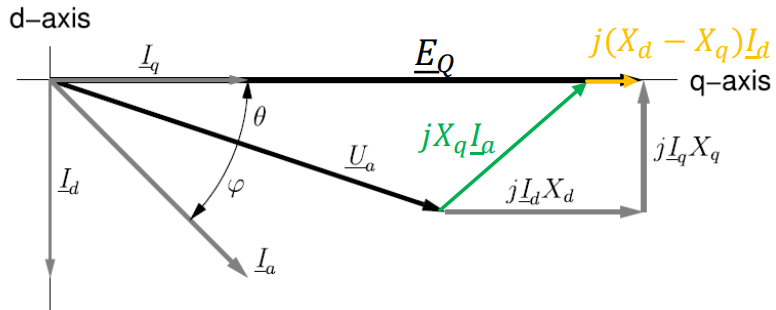
\includegraphics[width=\linewidth]{src/sp phasor diagram.png}
\end{wrapfigure}
% $u_x=-Ri_x-\frac{d\lambda_x}{dt}, \lambda_{x}=(L_s+M_s)i_x+\underbrace{\omega M_fI_f\sin(\omega t+\theta_{d0}-\rho_x)}_{=e_x'=\sqrt{2}|E_i|\cos(\omega t+\theta-\rho_x)}$ \\
\textbf{sp}: $E_Q=U_a+(R+jX_q)I_a=|E_Q|\angle\theta$ and $I_d=|I_a|\cos(\theta+\frac{\pi}{2}+\varphi)\angle(\theta+\frac{\pi}{2})$ to get $E_i=U_Q+j(X_d-X_q)I_d$. \textbf{rr}: $X_d=X_q$ so $E_i=U_a+jX_dI_a$ \\
\textbf{internal voltage magn.}: $|E_i|=\omega M_fI_f/\sqrt{2}$. \\
\textbf{active power control}: only changes with $T_m: \\ P=U_tE_i/X_d\sin\theta$. \\
\textbf{reactive power control}: with $I_f$, $Q=U_t/X_d(E_i\cos(\theta) - U_t)$. \\
\textbf{modes of operation}: over-excited (supplies $Q,\varphi<0, E_i\cos(\theta)>U_t$, like capacitor), unity power factor, under-excited. $i_{f,o}>i_{f,unity}>i_{f,u}$. \\
\textbf{motor operation}: $|\varphi|>90^\circ,\theta<0$ \\
\textit{example}: increase $i_f\Rightarrow$ higher $E_i, Q, pf$, over-excited, same $P$ as $\theta$ compensates. AVR adapts $I_f$ to keep $U_a$ close to $V_{ref}$.

\subsection{operational limits}
\begin{figure}[H]
    \centering
    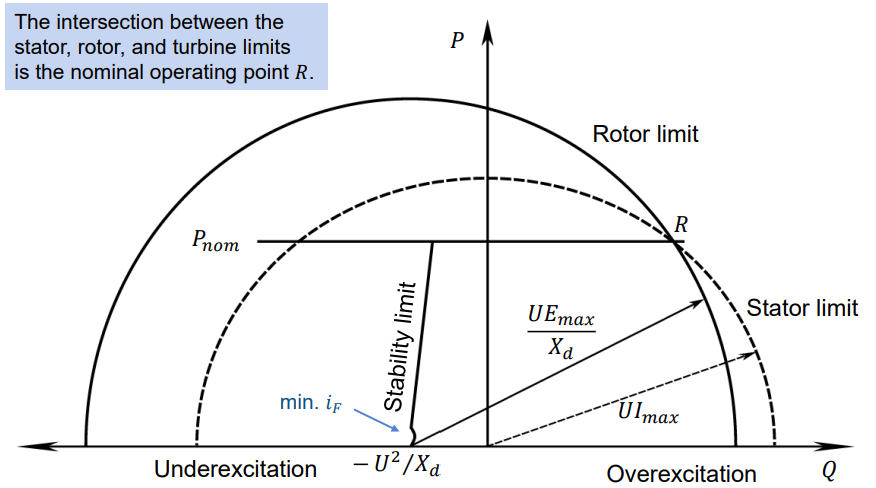
\includegraphics[width=1\linewidth]{src/capability curve.png}
\end{figure}
\vspace{-.5cm}

\textbf{Prime-Mover}: maximum mechanical power of turbine $P_{nom}$ \\
\textbf{Stator winding}: max. current the stator can withstand w.o. damage to insulation. $S^2=(UI_{max})^2\rightarrow$ described radius of $UI_{max}$\\
\textbf{Rotor winding}: maximum DC current the field winding can withstand $P^2+\left(Q+\frac{U^2}{X_d}\right)^2=\left(\frac{U E_{\max }}{X_d}\right)^2$ \\
\textbf{Rotor-angle stability}: for rr: $\theta<90^\circ$, for sp: $\theta<20^\circ$. \\
\textbf{end/region stator heating}: for under-excited steam generators, armature reaction \\
\textbf{Minimum field current}: at under-excitation, very low active power may lead to loss of sync. \\

\newpage

\subsection{saturation and Open Circuit Curve $U_{a,OC}(I_f) (OCC)$}
pre:$E_{ag}=U_a+I_a(R+jX_l)$, $I_a=\left((P+jQ)/U_a\right)^*$
\begin{wrapfigure}{l}{0.3\linewidth}
    \centering
    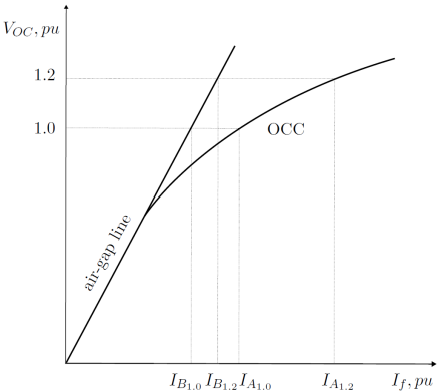
\includegraphics[width=\linewidth]{src/saturation.png}
\end{wrapfigure}
more evident at high $I_F$ values \\
$S_{1.0}=\frac{I_{A1.0}-I_{B1.0}}{I_{B1.0}}, S_{1.2}=\frac{I_{A1.2}-I_{B1.2}}{I_{B1.2}} $, $K_d=1/(S_x+1)$. saturation factor is $K_d=\frac{1}{1 + sat(\lambda_{ag})}=\frac{1}{1 + sat(|E_{ag}|)}$. for \textbf{rr}: $I_f=|E_i^{(s)}|/K_d\cdot I_{B1.0}=I_{f,pu}\cdot I_{B1.0}$ where $X_d^{(s)}=X_l+K_d(X_d-X_l)$. for \textbf{sp}: add. $X_q^{(s)}=X_l+K_q(X_q-X_l)$, $E_i^{(s)}=U_a+I_a\left(R+jX_q^{(s)}\right)+jI_d(X_d^{(s)} - X_q^{(s)})$ 
\vspace{-.3cm}
\begin{figure}[H]
    \centering
    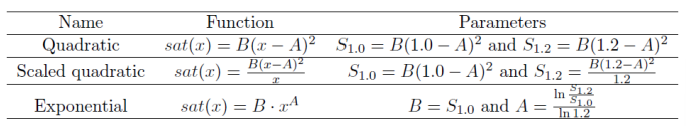
\includegraphics[width=\linewidth,right]{src/saturation functions.png}
\end{figure}
\vspace{-2cm}
\hspace{-2cm}
\textbf{saturation in $q-$axis.} \textbf{rr}: $K_q=K_d$.
3 options for \textbf{sp}: 1. $K_q\approx1$ . 2. $K_q=1/(1+X_q/K_d sat(x))$ or 3. $K_q\approx K_d$ same sat. in both axes.
\textbf{steps:}
\begin{enumerate}
    \item get $A,B$ via $S_{1.0},S_{1.2}$ (quadratic, exp., ...)
    \item compute $E_{ag}$ from $U_a,I_a$. Then calc. $K_d=1/(1 + sat(|E_{ag}|))$
    \item get $X_d^{(s)}$. get $E_i^{s}$. get $I_{f,pu}$
\end{enumerate}

\section{Fault Analysis}

\subsection{transients on a transmission line}
short circuit occurs when line is unloaded. why important? circuit breaker needs to be designed based on this value.
\begin{wrapfigure}{l}{0.5\linewidth}
    \centering
    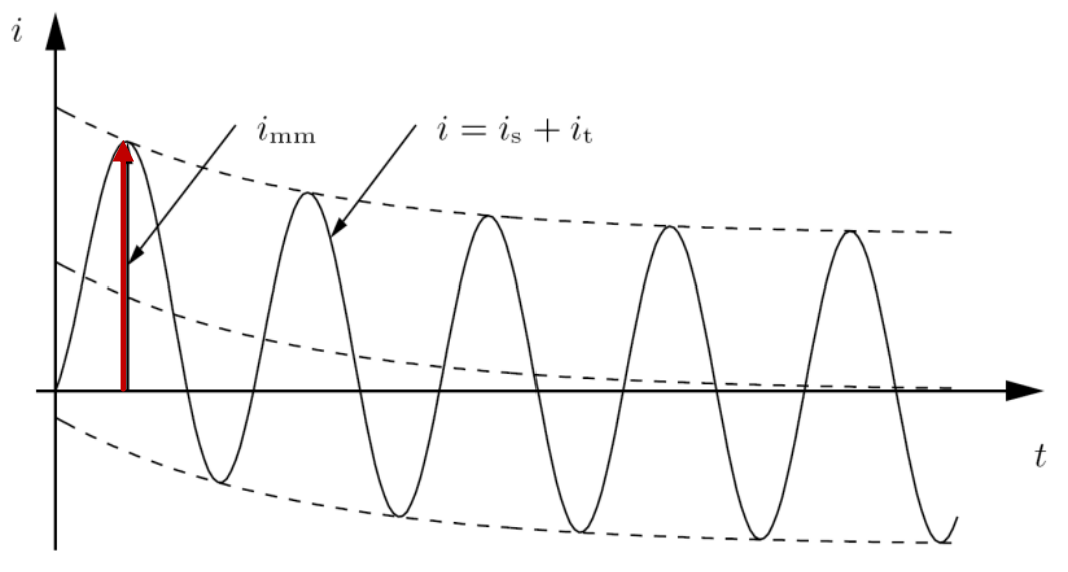
\includegraphics[width=\linewidth]{src/trans_line_SC.png}
\end{wrapfigure}
$i_s$ symmetrical short circuit current \\
$i_t$ DC off-set current \\
$i_{mm} \leq 2\frac{\sqrt{2}U}{|Z|}$ maximum momentary short circuit current.

\subsection{Short Circuit on Synchronous Machine}
right after fault: $U_a\rightarrow 0$, generator no longer at equilibrium and accelerates $(\omega_r'>\omega_r)$, currents induced in damper windings: 
\begin{figure}[H]
    \centering
    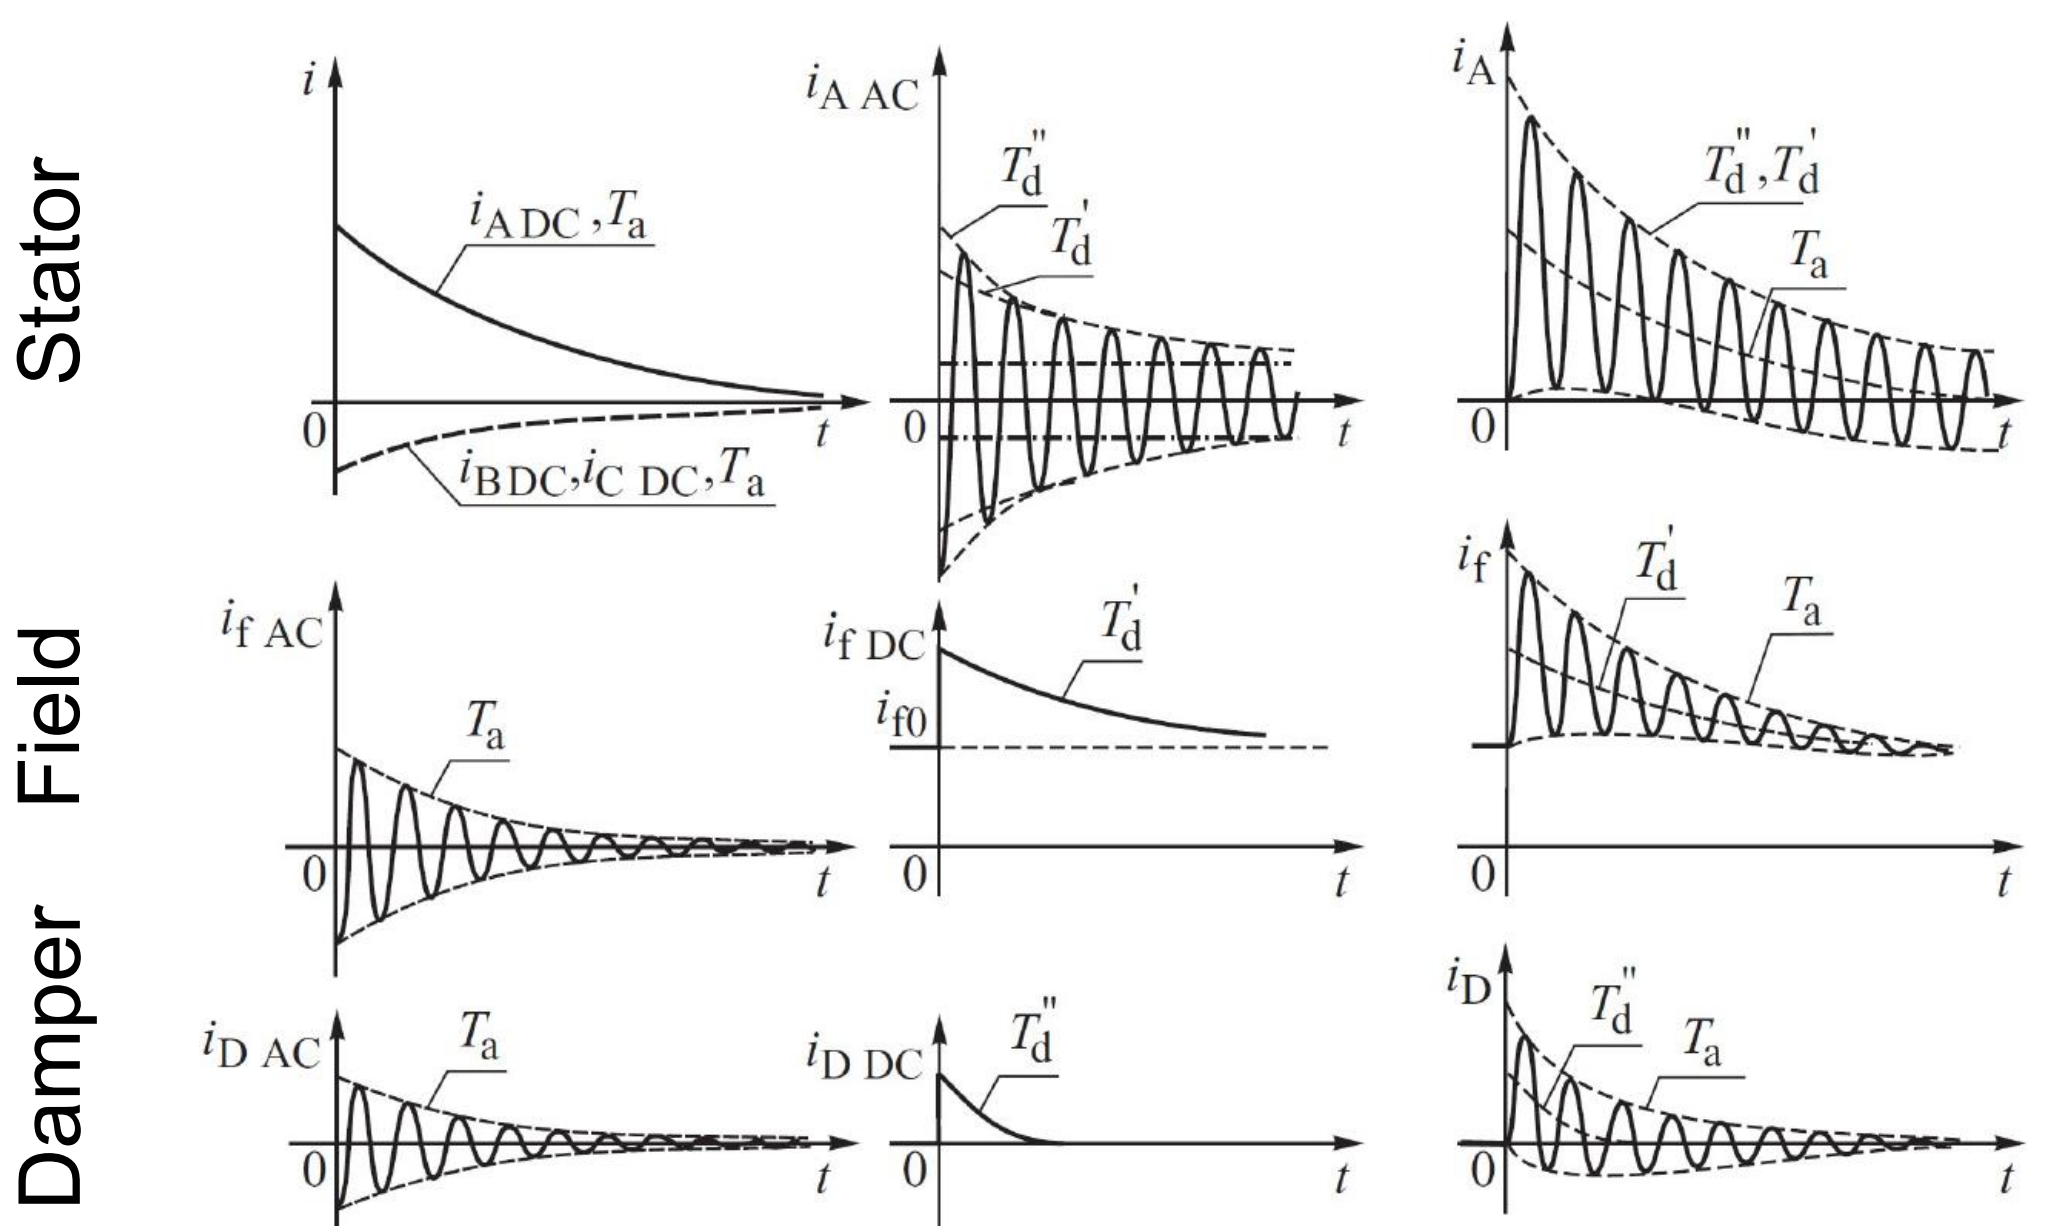
\includegraphics[width=1\linewidth]{src/sync_machine_SC.png}
\end{figure}
with $T_d''\prime<T_d'<T_a$ the sub-transient, transient and steady-state time constants. \\
during sub-transient: $X_d^{\prime \prime} \approx X_l+\frac{1}{1 / X_{m d}+1 / X_{l f}+1 / X_{l D}}$, during transient: $X_d^{\prime} \approx X_l+\frac{1}{1 / X_{m d}+1 / X_{l f}}$ the currents in damper windings have died out. \\
in steady state: $X_d=X_l + X_{md}$.

\subsection{Short Circuit Computations: Superposition Technique}
assume fault at node i, $\mathbf{Y\cdot U = I}$: \\
with $\mathbf{Y}$ nodal admittance matrix \\
$\mathbf{U} = \underline{U}_j$ if $j\neq i$ else $0$. \\
\begin{figure}[H]
    \centering
    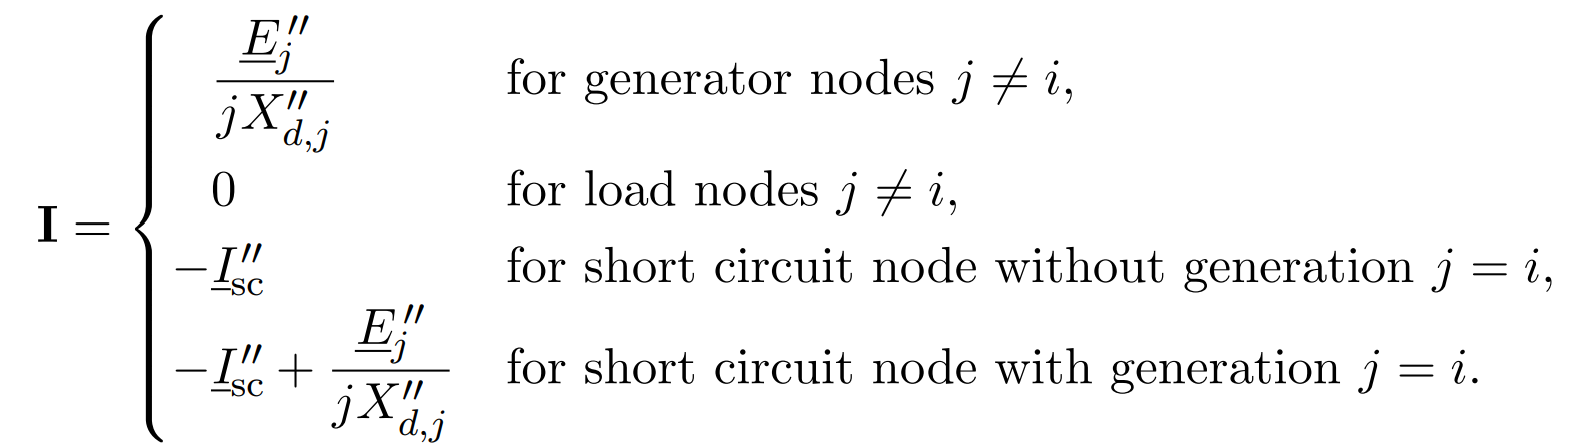
\includegraphics[width=1\linewidth]{src/SC_computation_I.png}
\end{figure}
\textbf{Main idea:}
\begin{figure}[H]
    \centering
    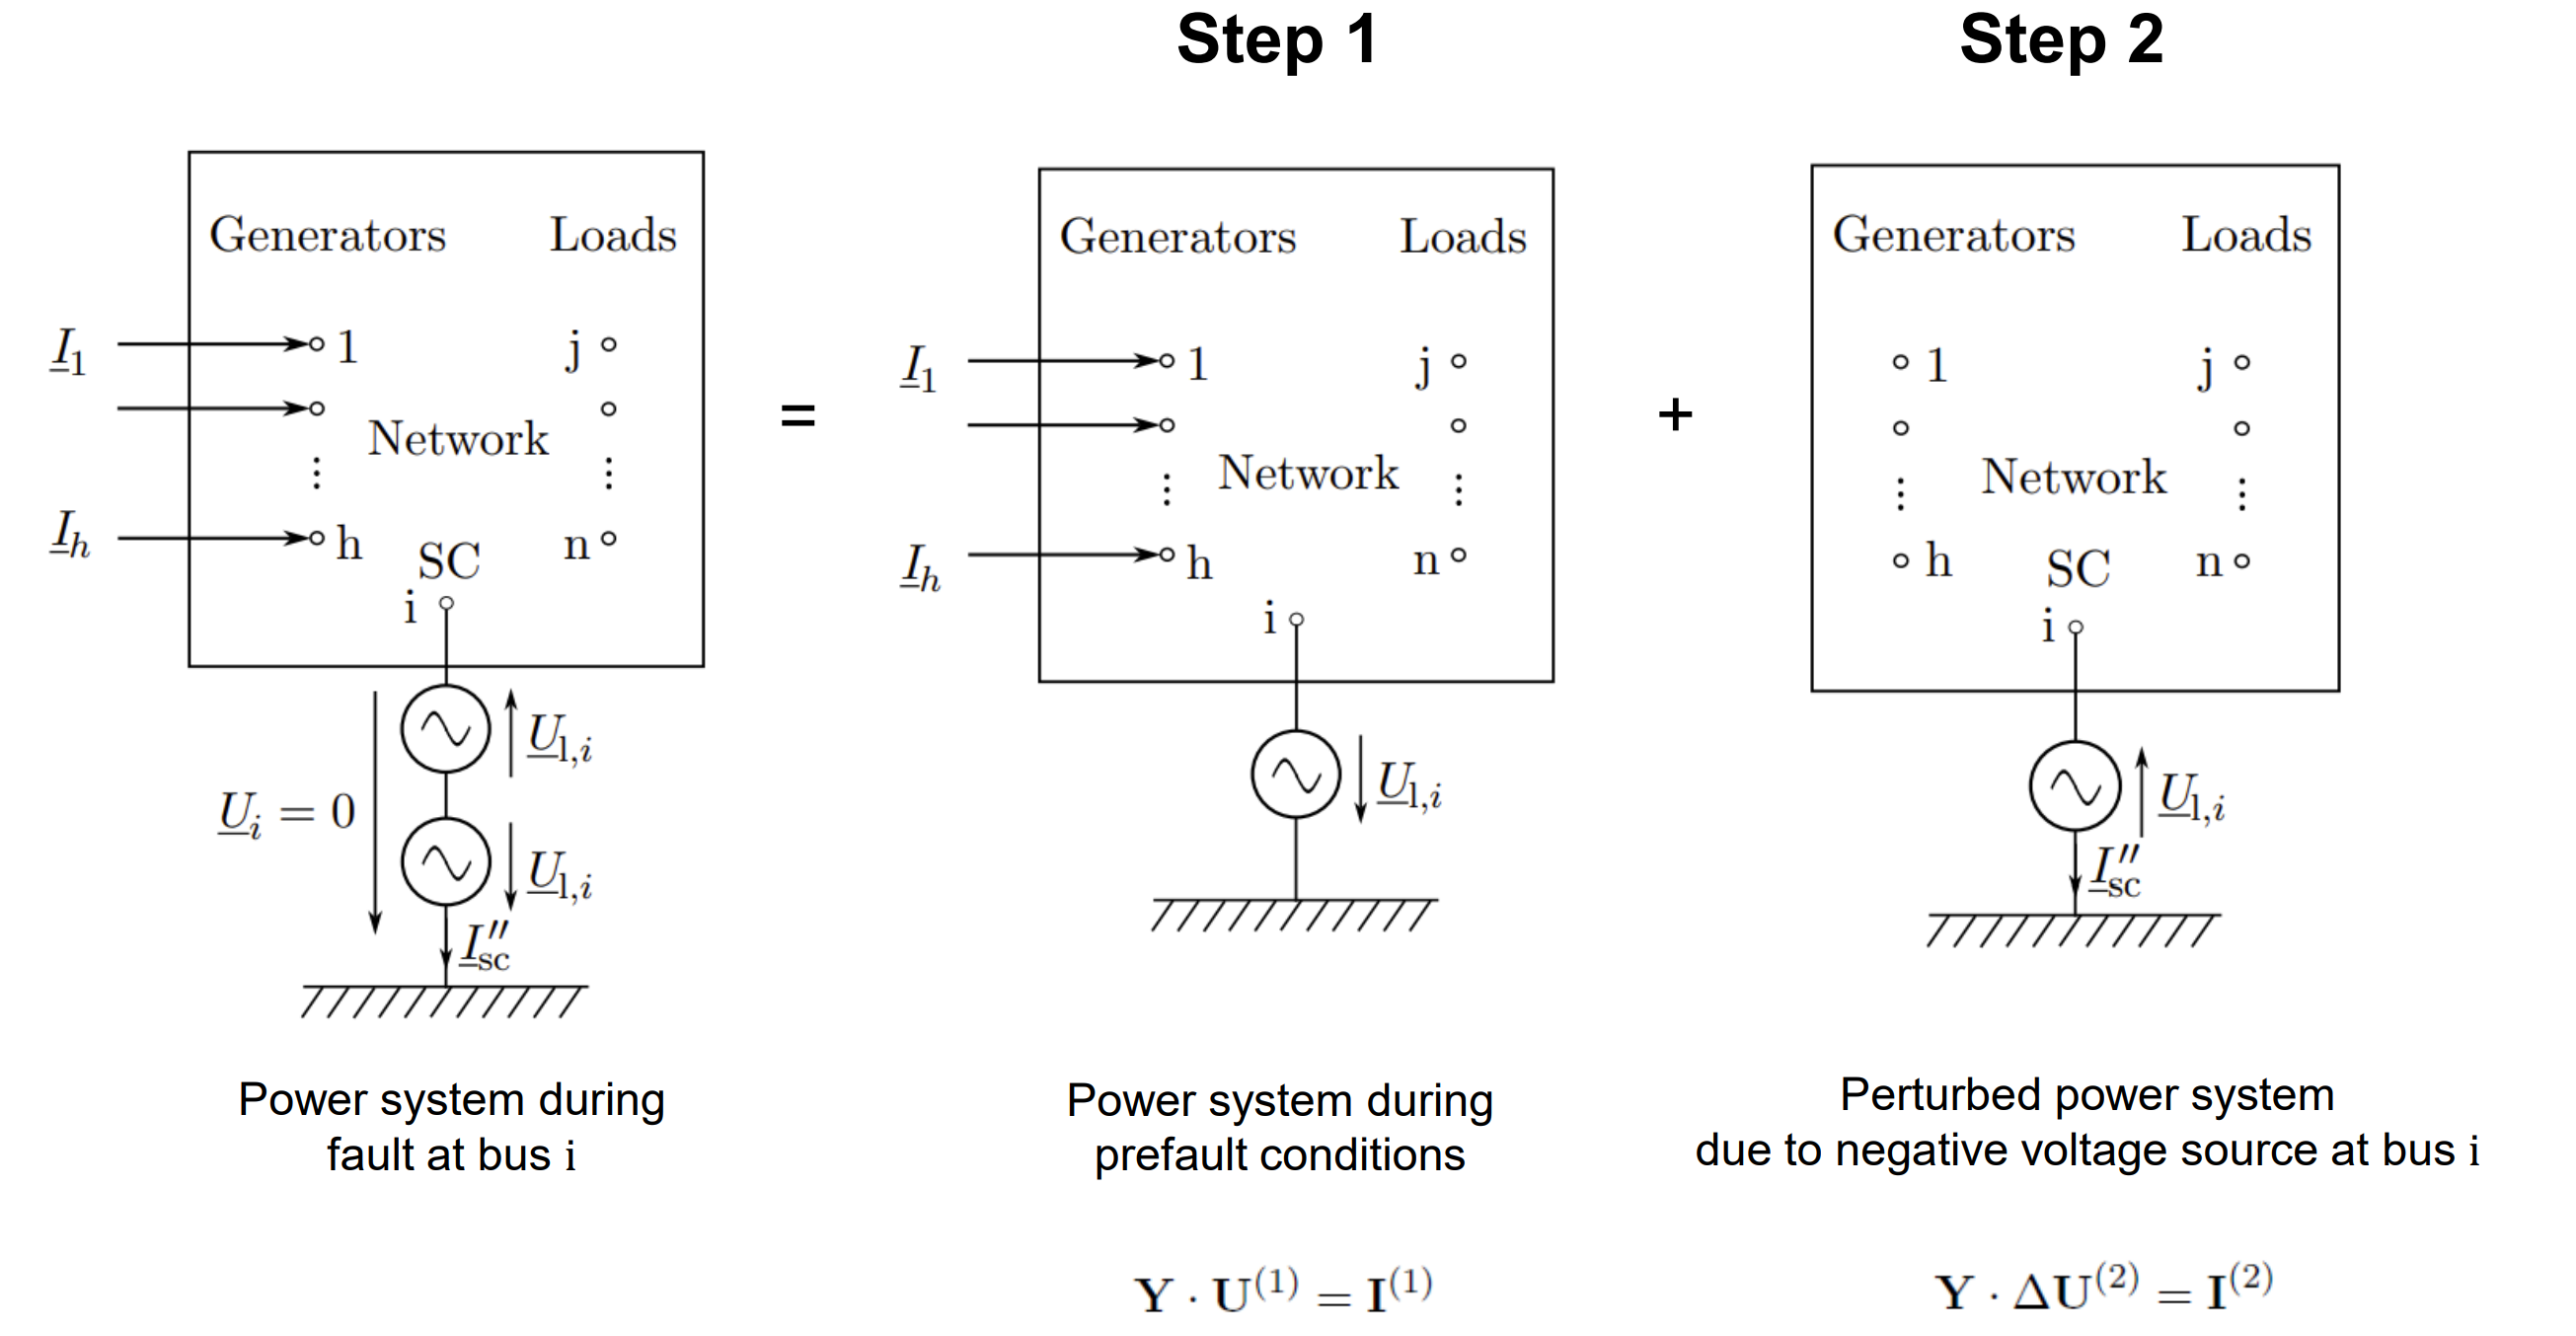
\includegraphics[width=1\linewidth]{src/superposition_tech_SC.png}
\end{figure}
\textbf{1. step}: calculate all pre-fault voltages (standard power flow analysis)

\textbf{2. step}: insert voltage $U_{1,i}$ in reverse direction at short circuit node. all currents/withdrawals by gen's/motors are 0, only short circuit is present. thus $\underline{I_{SC}'' = \frac{U_{1,i}}{Z_{ii}}}$ where $Z_{ii}$ is the i-th element of the impedance matrix $\mathrm{Z=Y^{-1}}$ or Thevenin equivalent impedance as seen from node $i$. Advantage of this approach: $\mathrm{Z}$ stays same regardless of SC location, can calculate $\underline{I_{SC}''}$ at any location with $\mathrm{Z}$.

\subsection{Thevenin Equivalent Method}
\begin{wrapfigure}{r}{0.5\linewidth}
    \centering
    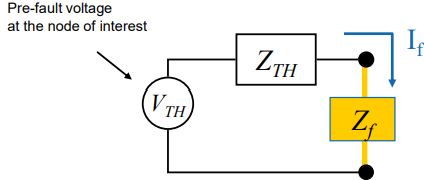
\includegraphics[width=\linewidth]{src/Thevenin Equivalent Method.png}
\end{wrapfigure}
for small test systems only, quick approx. of $\underline{I}_{SC}"$, ignores pre-fault currents. ($Z_f=0$ most times): \\
$I_f=\frac{V_{TH}}{Z_{TH}+Z_f}$ 

\subsection{Short Circuit Capacity (SCC)}

$$\mathrm{SCC}_i = \sqrt{3}U_{b}|\underline{I}_{f_{i}}|$$
where $U_b$ is the L-L base voltage in kV and $\underline{I}_{f_{i}}$ is the fault current in kA, thus $\mathrm{SCC}$ in MVA.


\section{Symmetrical Components and Unbalanced Faults}
1. Transform $\mathrm{RST}\overset{S}{\Rightarrow}120$: $\mathbf{I_{120} = S\cdot I_{RST}}, \mathbf{U_{120} = S\cdot U_{RST}}$ 2. solve in $120$ form. 3. back-transform: $\mathbf{I_{RST} = T\cdot I_{120}}$ \\ $T=\left(\begin{array}{ccc}
1 & 1 & 1 \\
a^2 & a & 1 \\
a & a^2 & 1
\end{array}\right), S=\frac{1}{3}\left(\begin{array}{ccc}
1 & a & a^2 \\
1 & a^2 & a \\
1 & 1 & 1
\end{array}\right), a=e^{j\cdot 120^\circ}$
note: saved as \texttt{tt} and \texttt{ss} in Ti-npsire
\begin{figure}[H]
    \centering
    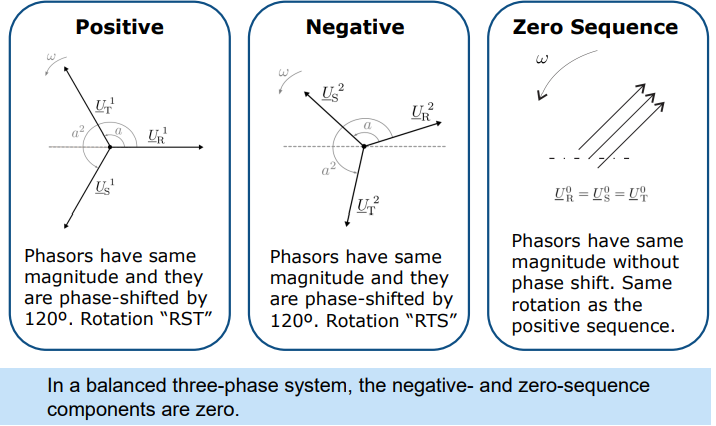
\includegraphics[width=1\linewidth]{src/symmetrical components.png}
\end{figure}
\vspace{-.5cm}
% zero sequence system and fault analysis plot should be given in exam.
\textbf{positive sequence}: single-phase equ. of balanced system. $Z_1$ including all passive elements is independent of $Z_E$. all neutral elements considered connected. voltage source positive. Delta- has to be transformed to Y.
\textbf{negative sequence}: voltage source is zero (short circuit), $Z_2=Z_1$. rest same as in positive sequence.
\textbf{zero sequence}: sources/generators are 0. $Z_{np}=3Z_E$. 

\subsection{Single-Phase-to-Ground Fault}
$R\cdot I_R=U_R, I_S=I_T=0$ and $I_1=I_2=I_0=\frac{E_1}{Z_1+Z_2+Z_0+3R}$\\
fault current: $I_f=I_R=3I_1$ where $E_1=E_R$

\subsection{Two-Phase Short Circuit Without Ground Contact}
$I_R=0,I_S=-I_T,U_S-U_T=R\cdot I_S$. transforming: $I_1=-I_2,I_0=0,U_1-U_2=R\cdot I_1$ \\
fault current: $I_f=I_s=a^2I_1+aI_2+I_0 = -j\sqrt{3}\frac{E_R}{Z_1+Z_2+R}$ where $E_R=E_1$

\subsection{Three-Phase Short Circuit}
$U_i=R\cdot I_i$ for $i=\{R,S,T,1,2,0\}$ \\
fault current: $I_f=I_R=\frac{E_R}{Z_1+R}$


\section{Operation Principles}
\subsection{types of instabilities}
\begin{itemize}
    \item $f$ instability: not matching load and generation globally
    \item $V$ instability: inacceptable voltage at 1 or more buses (a.k.a. load instability, e.g. motors)
    \item transient $\theta$ instability: loss of synchronism (after large disturbance)
    \item Small-Signal Angular ($\theta$) Instability: loss of synchronism (after small disturbance)
\end{itemize}

\begin{figure}[H]
    \centering
    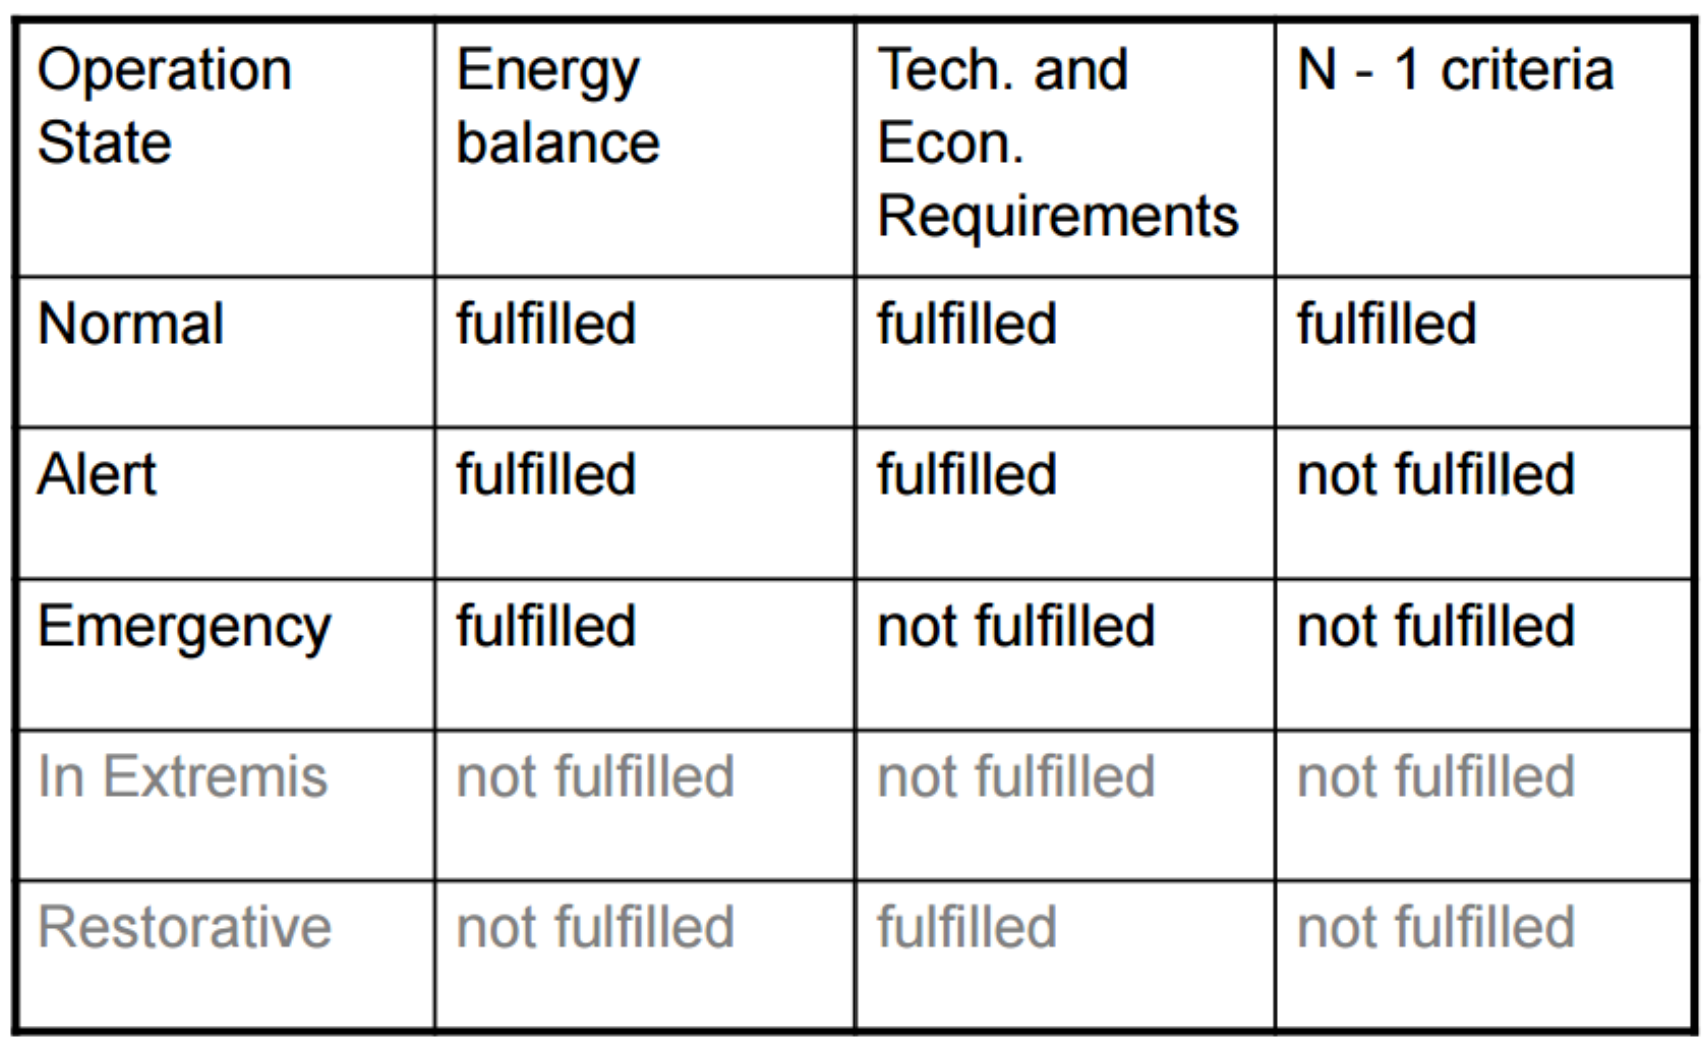
\includegraphics[width=.9\linewidth]{src/operation_table.png}
\end{figure}

% todo
\vspace{4cm}

\section{operational states}



\begin{wrapfigure}{r}{0.3\linewidth}
    \centering
    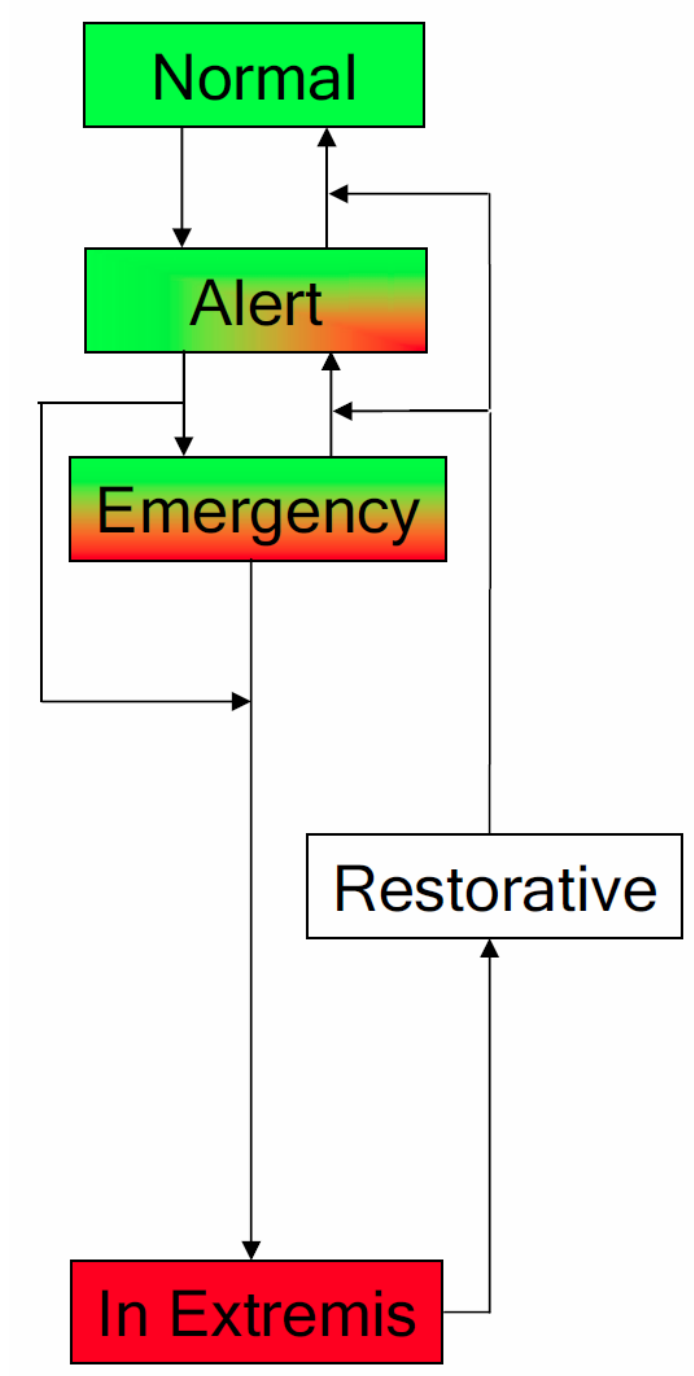
\includegraphics[width=\linewidth]{src/operation_sketch.png}
\end{wrapfigure}
\textbf{Alert}: variables still within acceptable range, but system is weakened (N-1 state).
\textbf{Emergency}: Some system variables are outside of
acceptable range.
\textbf{Extremis}: partial or total blackout. 
\textbf{Restoration}: Energizing of the system or its parts
and reconnection and resynchronization of system
parts

\subsection{day-ahead operation planning}
based on electricity markets. production is checked against potential violations $\rightarrow$ generation schedule may have to be adjusted

\subsection{short term planning}
$\tau~$ in order of several days to weeks. E.g. maintenance of grid components

\subsection{long term planning}
load forecasting and estimating peak demand / expected generation. \\
adequacy assessment: loss of load / unnerved energy \\
security assessment: simulation of dangerous situations, determination of operational limits \\
short-circuit analysis: study possible short circuit currents \\

\subsection{general market structure}
\textbf{participants}: generators, loads, balancing group, transmission system operator, regulator \\
\textbf{types of markets}: imbalance / energy-only market

\section{State Estimation (SE)}
\textbf{goal}: most likely state $\mathbf{x=[U,\theta]^T}\in \mathcal{R}^n$ of system given a set of measurements $\mathbf{z}$. careful: remove ref. angle $\theta_i=0$ from $\mathbf{x}$.

\subsection{measurements}
\begin{itemize}
    \item voltage magnitudes
    \item voltage angles
    \item current magnitudes
    \item power flows
    \item generator outputs, loads
    \item circuit breaker, transformers
\end{itemize}

\subsection{to consider}
\textbf{topology processor}: get one-line diagram from status data (circuit breaker, switches)

\textbf{observability analysis}: identify unobservable branches

\textbf{state estimation solution}: determines optimal estimate for the system state

\textbf{data filtering}: exclude NaN, unrealstic values, ect.

\textbf{Parameter and Structural Error Processing}: estimates various network parameters

general goal: \textbf{weighted least square estimation}
$$\min _{\mathbf{U}, \boldsymbol{\theta}} J(\mathbf{x})=\sum_i W_{i i}\left(z_i-h_i(\mathbf{U}, \boldsymbol{\theta})\right)^2$$

\subsection{notation}
\begin{itemize}
    \item $x_i$ – states, $z_i$ – measurements
    \item $e_i$ – measurement errors, Gaussian probability dist.
    \item $\mu_i$ – mean/expected value, $\sigma_i$ – standard deviation
    \item $W_{ii}$–weight for meas. accuracy, $\mathbf{W} = \text{diag}(W_{ii}) = \mathbf{R}^{-1}$
    \item $r_i$ – residuals of measurements from expected value
    \item $h_i(x)$ – measurement function, e.g. $P_{12}(\mathbf{x})=U_1^2g-\dots$
    \item $\mathbf{H}(x)=\frac{\delta h(x)}{\delta x}$ measurement Jacobian 
    \item $J(x)$ – optimization objective function
    \item $\mathbf{g}(x)$ – partial derivative of $J(x)$ with respect to $x$
    \item $\mathbf{G}(x)$ – the gain matrix (an approximation of the partial derivative of $\mathbf{g}(x)$ with respect to $x$)
\end{itemize}

\subsection{solving it}
\textbf{Maximum Likelihood Estimation} \\
assume errors are stochastic with zero mean gaussian, i.i.d. \\
build likelihood function: $f_m(\mathbf{z})=f(z_1)\cdot f(z_2)\dots f(z_m)$
$$
    \mathrm{argmax}_{\mu_i} \log f_m(\mathbf{z}) \\
    \text{ is equivalent to }\underset{\mu}{\min}\sum_{i=1}^{m}\left(\frac{z_i-\mu_i}{\sigma_i}\right)^2
$$
But what is $\mu_i$? it is our model function $h_i(\mathbf{x})$. \\
Thus equivalent to solve \textbf{weighted least square estimation} of
\begin{flalign*}
& \min _{r_i} J(\mathbf{x})=\sum_i W_{i i}r_i^2, \quad W_{ii}=1/\sigma_i^2\\
\text{s.t. } & r_i=z_i - h_i(\mathbf{x})
\end{flalign*}

\subsubsection{solution for WLS estimation}
\[
\Delta \mathbf{x}^{k+1} = 
\left( \mathbf{H}^\top(\mathbf{x}^k) \cdot \mathbf{W} \cdot \mathbf{H}(\mathbf{x}^k) \right)^{-1} \cdot 
\left( \mathbf{H}^\top(\mathbf{x}^k) \cdot \mathbf{W} \cdot 
\left( \mathbf{z} - \mathbf{h}(\mathbf{x}^k) \right) \right)
\]

\[
\mathbf{x}^{k+1} = \mathbf{x}^k + \Delta \mathbf{x}^{k+1}
\]

\begin{enumerate}
    \item Start iterations, set the iteration index $k = 0$.
    \item Initialize the state vector $\mathbf{x}^k$, typically as a flat start.
    \item Calculate the gain matrix $\mathbf{G}(\mathbf{x}^k) = \mathbf{H}^\top(\mathbf{x}^k) \cdot \mathbf{W} \cdot \mathbf{H}(\mathbf{x}^k)$.
    \item Calculate the right-hand side $\mathbf{g}(\mathbf{x}^k) = -\mathbf{H}^\top(\mathbf{x}^k) \cdot \mathbf{W} \cdot 
    \left( \mathbf{z} - \mathbf{h}(\mathbf{x}^k) \right)$.
    \item Solve for the update $\Delta \mathbf{x}^{k+1} = -\mathbf{G}(\mathbf{x}^k)^{-1} \cdot \mathbf{g}(\mathbf{x}^k)$.
    \item Test for convergence, i.e. is $\max \lvert \Delta \mathbf{x}^{k+1} \rvert \leq \epsilon$ ?
    \item If no, update $\mathbf{x}^{k+1} = \mathbf{x}^k + \Delta \mathbf{x}^{k+1}$, set $k = k + 1$ and go to step 3.
\end{enumerate}
note that:
\[
\frac{-\partial J(\mathbf{x})}{\partial \mathbf{x}} = \underbrace{\begin{bmatrix}
    \frac{\partial h_1(\mathbf{x})}{\partial x_1} & \frac{\partial h_2(\mathbf{x})}{\partial x_1} & \cdots & \frac{\partial h_m(\mathbf{x})}{\partial x_1} \\
    \frac{\partial h_1(\mathbf{x})}{\partial x_2} & \frac{\partial h_2(\mathbf{x})}{\partial x_2} & \cdots & \frac{\partial h_m(\mathbf{x})}{\partial x_2} \\
    \vdots & \vdots & \ddots & \vdots \\
    \frac{\partial h_1(\mathbf{x})}{\partial x_n} & \frac{\partial h_2(\mathbf{x})}{\partial x_n} & \cdots & \frac{\partial h_m(\mathbf{x})}{\partial x_n}
\end{bmatrix}}_{\mathbf{H}^\top} 
2\mathbf{W}
\begin{bmatrix}
    z_1 - h_1(\mathbf{x}) \\
    z_2 - h_2(\mathbf{x}) \\
    \vdots \\
    z_m - h_m(\mathbf{x})
\end{bmatrix}
\]
issues: $\mathbf{G}$ may not be invertible. Use \textbf{Cholesky factorization} to solve it.

\subsection{bad data detection}
$\chi^2$-Test. is effective if single bad measurement is 1) not a critical meas. and 2) does not belong to critical pair. procedure:
\begin{enumerate}
    \item solve WLS estimation
    \item carry out $\chi^2$ test: $J(\mathbf{x})\geq \chi^2_{\textbf{df},p}$. negative? $\Rightarrow$ stop
    \item compute normalized residuals $\max{r_i^N}$
    \item if $\max{r_k^N}>$thresh. $\Rightarrow$ eliminate $k$
    \item repeat
\end{enumerate}
degrees of freedom: $\textbf{df}=\#\text{meas.}-\#\text{states}$. $p$: usually $95\%$

\section{Observability Analysis}
fully obs.: all voltage phasors uniquely estimated using meas. \\
unobs.: power flow/voltages of $\geq1$ bus cannot be determined \\
obs. island: unobs. branches connect obs. islands \\
consider state $\mathbf{x}=\left[x_1\dots x_n\right]^T\in \mathcal{R}^n$. if no meas. err.: $\mathbf{Hx=z}$ generally has multiple sol. $\mathbf{x^*=x^P+Z\eta}$ where $\mathbf{Z}=\mathrm{ker}(\mathbf{H}):=\mathbf{ZH}=0$, $\eta$ vector of params. $\mathbf{H}\in\mathcal{R}^{m\times n}$ \\
if $\mathbf{Z}$ null: observable. otherwise: unobs. \\
for row $i:x_i^*=x_i^P + \sum_{j=1}^k Z_{ij}\eta_j \quad\forall i$ $\Rightarrow$ state $x_i$ observable if $Z_{ij}=0\quad\forall j$

\subsection{other issues}
parameters of system assumed differ from actual value/vary during operation of system $\Rightarrow$ \textbf{parameter errors} \\
\textit{consequence}: Significant adverse impact on SE results \\
status of circuit breaker is determined incorrectly $\Rightarrow$
locally incorrect bus/branch model $\Rightarrow$ \textbf{topological error} \\
\textit{types}: 1) substation conf. err. e.g. CB linking busbars and 2) branch status error. \\
2) solution: state vector augmentation by $k$ \textit{branch status} state, i.e. if non-zero impedance suspected at $i\leftrightarrow j$. thus: \\
\resizebox{\hsize}{!}{$P_{i j}(k)=k P_{i j}=k\left\{U_i^2\left(g_{i j}^{s h}+g_{i j}\right)-U_i U_j\left(g_{i j} \cos \theta_{i j}+b_{i j} \sin \theta_{i j}\right)\right\}$} \\
\resizebox{\hsize}{!}{$P_i(k)=\sum_{\substack{m=1 \\ m \neq j}}^n P_{i m}+k P_{i j}=U_i \sum_{\substack{m=1 \\ m \neq j}}^n U_m\left(G_{i m} \cos \theta_{i m}+B_{i m} \sin \theta_{i m}\right)+k P_{i j}$} \\
start with $k^{(0)}=0.5$ and do WLS.



\section{Monitoring and Protection}
\textbf{SCADA}: Supervisory Control and Data Acquisition \\
SCADA functions include:Data acquisition, Remote control, Human-machine interface, Historical data analysis, Report writing \\
\textbf{EMS}: Energy Management System. processes data from SCADA. \\
EMS capabilities: Network Configuration/Topology Processor, State Estimation, Contingency Analysis, Optimal Power Flow

\subsection{Protection}
purpose: protect power system by removing faulted element (to minimize damage). \\
general requirements: \textbf{Reliability, Selectivity, Speed, Sensitivity} \\

\subsubsection{Protection Systems}
two types: \textbf{absolute selectivity}. can only detect internal faults. \textbf{relative selectivity}. can identify external faults additionally. \\
\textbf{Overcurrent Protection} (relative) \\
trip circuit breaker if RMS current exceeds threshhold \\
are inappropriate for time critical applications $\Rightarrow$ offer only limited selectivity and coordination. Advantage: simplicity, i.e. low production and installation cost. Used mainly in distribution networks for overhead lines and cables \\
\textbf{Differential Protection} (absolute) \\
Determines sum of complex values of currents measured at both
ends of protected object. If sum exceeds predefined differential current value => tripping
signal is sent. Differential protection in transmission lines is vulnerable to
communication loss and delay $\Rightarrow$ high requirements on reliability
and speed of communication

\section{Appendix}
\section{basics}
$U_{pp}=\sqrt{3}U_{pn}$ ($p$: phase, $n$: neutral). for $\sin/\cos$: $U_\mathrm{rms}=\frac{\hat{U}}{2}$. \\
inductance: $u_L=L\frac{di}{dt}$ capacitance: $i_C=C\frac{du}{dt}$. $P=UI\cos\varphi$, $Q=UI\sin\varphi$. $S=UI^*=3U_{pp}I_{pp}^*$. \\
in steady-state, for all times $t$: $i_R+i_S+i_T=0=u_R+u_S+u_T$. \\
Wye-Delta conversion: $Z_d=3\cdot Z_y$.

\subsection{update formula $f(\omega_{k-1})$ for full BFS power flow} \label{full_NRM_f}
\begin{mdframed}
1. $\underline{\tilde{E}}_k=\underline{E}_{k-1}+Z_k\left(\frac{1}{2} Y_k \underline{E}_{k-1}-\underline{I}_k\right)$ \\
2. $\tilde{\tilde{I}}_k^{\prime}=\frac{1}{2} Y_k\left(\underline{\tilde{E}}_k+\underline{E}_{k-1}\right)-\underline{I}_k $ \\
3. $\underline{I}_{k+1}=\underline{I}_{G k}+\underline{\tilde{I}}_{C k}-\tilde{I}_{L k}-\underline{I}_k^{\prime}-\sum_{j \in A_k} \underline{I}_j$ \\
\end{mdframed}




% \begin{figure}
%     \centering
%     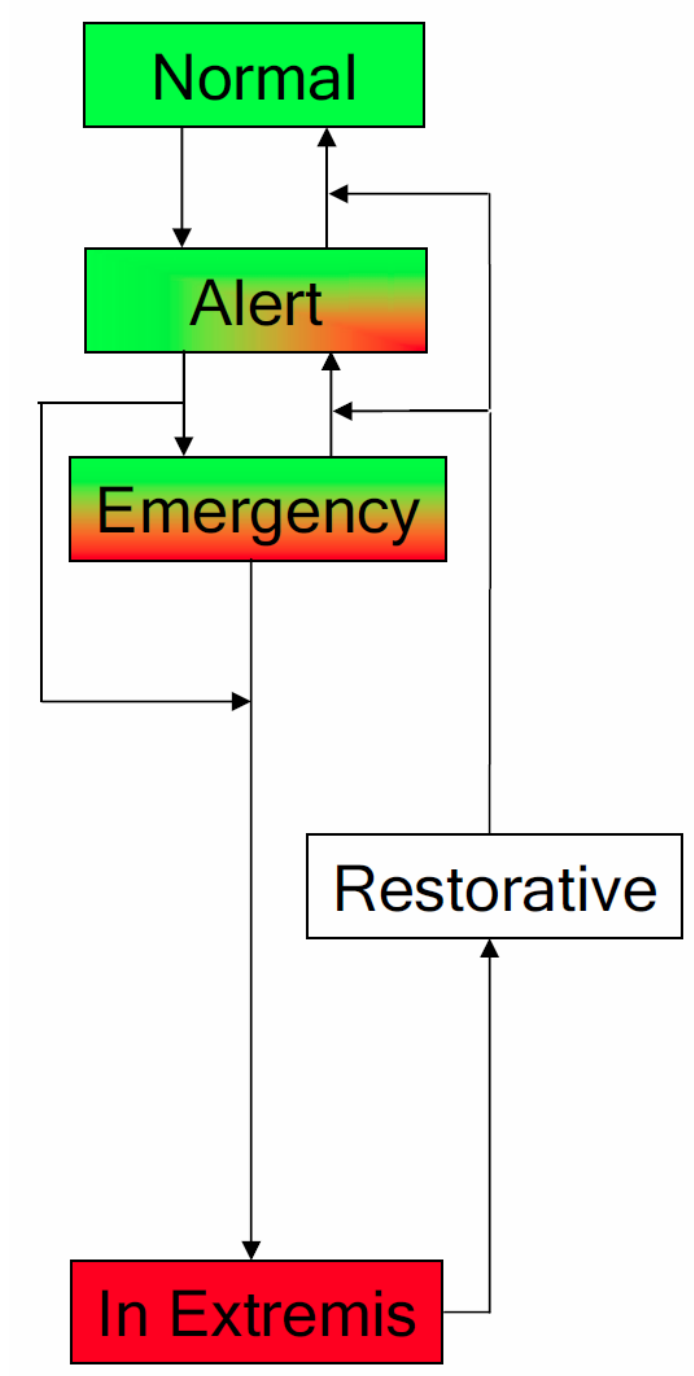
\includegraphics[width=0.5\linewidth]{src/operation_sketch.png}
% \end{figure}


\end{multicols*}
\end{document}